\chapter{Monte Carlo Methods}
\label{cha:Monte Carlo Methods}

As shown in the last chapter, Bayesian model comparison usually involves
computation of some integrations with respect to complex posterior
distributions. Only in very special situations, this can be resolved
analytically. In most cases, these integrations are approximated using
simulation techniques. In this chapter, we review some of the widely used
Monte Carlo methods with an emphasis on their applications to Bayesian
computation.

In Section~\ref{sec:Classical Monte Carlo} we introduce the basic idea of
Monte Carlo integration. Section~\ref{sec:Importance sampling} discusses the
importance sampling technique. Section~\ref{sec:Markov chain Monte Carlo}
reviews a class of important Monte Carlo algorithms, Markov chain Monte Carlo.
This chapter is concluded by Section~\ref{sec:Monte Carlo Discussion}, a
discussion on the reviewed algorithms and some other development in this area
that is not reviewed in detail.

\section{Classical Monte Carlo}
\label{sec:Classical Monte Carlo}

Classical Monte Carlo integration approximates the expectation of a function
$\varphi$ with respect to a (continuous) distribution $\pi$,
\begin{equation*}
  \Exp_{\pi}[\varphi(X)] = \int\varphi(x)\pi(x)\intd x
\end{equation*}
provided that the above expectation exists, by drawing identically
independently distributed (i.i.d.) samples from
$\pi$, say $\{X^{(i)}\}_{i=1}^N$, and approximating the expectation by the
empirical average,
\begin{equation}
  \hat\varphi_{\mc}^N = \frac{1}{N}\sum_{i=1}^N\varphi(X^{(i)}).
  \label{eq:vanilla mc}
\end{equation}
This method is also called \emph{vanilla} Monte Carlo or \emph{na\"\i ve}
Monte Carlo. The estimator $\hat\varphi_{\mc}^N$ converges almost surely to
$\Exp_{\pi}[\varphi(X)]$ when $N\to\infty$ by the Strong Law of Large Numbers
(\slln).

Clearly this method can only be applied when drawing samples directly from
the target distribution $\pi$ is possible. There are a few ways to draw
random variates from a reasonably well behaved distribution. See
\cite[][chap.~2]{Robert:2004tn} on this topic. In many cases, simulation from
a distribution $\pi$ efficiently requires the evaluations of its density
function point-wise, or finding some easy to simulate distribution that
closely imitates $\pi$. In the context of Bayesian computation, the target
distributions are usually complex posteriors only known up to some
normalizing constants. And thus point-wise evaluation is not possible. In
addition, the high dimensional aspect of many models makes it near impossible
to find a distribution closely imitates the target. In addition, even when it
is possible, the accuracy of the estimator $\hat\varphi_{\mc}^N$ depends
heavily on the function $\varphi$.

For example, consider the approximation of the marginal likelihood (see
Section~\ref{sub:Bayes factor}),
\begin{equation*}
  p(\data|\calM_k) =
  \int f(\data|\theta_k,\calM_k)\pi(\theta_k|\calM_k) \intd \theta_k,
\end{equation*}
or equivalently,
\begin{equation}
  p(\data|\calM_k) = \Exp_{\pi}[f(\data|\theta_k,\calM_k)],
  \label{eq:prior expectation}
\end{equation}
where the expectation is taken with respect to the prior distribution
$\pi(\theta_k|\calM_k)$. It is possible to use samples from
$\pi(\theta_k|\calM_k)$, the prior distribution, to approximate the
integration. With samples generated from $\pi(\theta_k|\calM_k)$, say
$\{\theta_k^{(i)}\}_{i=1}^N$, we can approximate $p(\data|\calM_k)$ by,
\begin{equation}
  \widehat{p(\data|\calM_k)}_{\mc}^N
  = \frac{1}{N}\sum_{i=1}^N f(\data|\theta_k^{(i)},\calM_k).
\end{equation}
This estimator was studied in \cite{McCulloch:1991hj} and also mentioned in
\cite{Kass:1995vb}. However, this approach often results in large variances.
The likelihood function (and thus the posterior distribution) is often much
more concentrated than the prior distribution. And there may be a large
proportion of samples with small likelihood values and a few with high
values. For instance, consider the one-compartment \pet model (see
Section~\ref{sec:Application to positron emission tomography}) and
informative priors (see Section~\ref{sub:Choice of priors}). Using 100,000
samples from the prior distribution, the empirical mean and standard
deviation of the estimates from 100 simulations is $-40.9$ and $2.1$,
respectively for the simulated data. However when the dimension of the model
is increased by using a two-compartments model, the estimates have empirical
mean and standard deviation $-39.6$ and $12.6$, respectively. The variance is
too large for practical use of evaluating the Bayes factor. Similar problems
were also shown in \cite{McCulloch:1991hj}.

\section{Importance sampling}
\label{sec:Importance sampling}

The \emph{importance sampling} method is based on the observation of the
following identity,
\begin{equation}
  \Exp_{\pi}[\varphi(X)]
  = \int\varphi(x)\pi(x)\intd x
  = \int\varphi(x)\frac{\pi(x)}{\eta(x)}\eta(x)\intd x
  = \Exp_{\eta}\Square[bigg]{\varphi(X)\frac{\pi(X)}{\eta(X)}},
  \label{eq:impotance fundamental}
\end{equation}
where $\eta$ is a distribution with respect to which $\pi$ is absolutely
continuous and the two expectations are taken with respect to $\pi$ and
$\eta$, respectively. The above equation is termed \emph{importance
fundamental identity} in \cite{Robert:2004tn}. The distribution $\eta$ is
often called the \emph{proposal} or \emph{instrumental} distribution. Thus
given i.i.d\ samples $\{X^{(i)}\}_{i=1}^N$ from distribution $\eta$, the
expectation $\Exp_{\pi}[\varphi(X)]$ can be approximated by the following
importance sampling estimator,
\begin{equation}
  \hat\varphi_{\is}^N
  = \frac{1}{N}\sum_{i=1}^N\varphi(X^{(i)})\frac{\pi(X^{(i)})}{\eta(X^{(i)})}.
  \label{eq:is normalized}
\end{equation}
The above estimator converges almost surely to $\Exp_{\pi}[\varphi(X)]$ when
$N\to\infty$. However, its variance is not necessarily finite. In general, the
variance is finite if and only if, \cite[][sec.~3.3.2]{Robert:2004tn},
\begin{equation}
  \int(\varphi(x))^2\frac{(\pi(x))^2}{\eta(x)} < \infty.
\end{equation}
To access the above inequality, evaluating a more complex integration than the
original problem is required. In \cite{Geweke:1989tm} two types of sufficient
conditions were mentioned. One is that $\pi/\eta$ is upper bounded and
$\var_{\pi}[\varphi(X)]$ is finite. Another is that the support is compact,
$\pi$ is upper bounded and $\eta$ is lower bounded by $\varepsilon > 0$.

Both $\pi$ and $\eta$ are often only known up to some normalizing constants,
which can be approximated with the same samples. This leads to the estimator,
\begin{equation}
  \hat\varphi_{\wis}^N
  = \frac{\sum_{i=1}^Nw^{(i)}\varphi(X^{(i)})}{\sum_{i=1}^Nw^{(i)}}
  \label{eq:is unnormalized}
\end{equation}
where $w^{(i)} \propto \pi(X^{(i)})/\eta(X^{(i)})$, and are termed the
\emph{importance weights}. This estimator also converges almost surely to
$\Exp_{\pi}[\varphi(X)]$ when $N\to\infty$. This estimator has a bias since
it is the ratio of two unbiased estimator. However, even when the normalizing
constants of $\pi$ and $\eta$ are both known, this estimator can be
preferable to $\hat\varphi_{\is}$ due to its possible smaller mean squared
error. In fact, \cite{Casella:1998tj} showed an example of using the Cauchy
distribution as the proposal distribution for the evaluation of expectations
under the Student~$t$ distribution, where for some functions, such as
$\varphi(x) = |x|$, $\hat\varphi_{\wis}^N$ can outperform
$\hat\varphi_{\is}^N$ considerably.

In general, the performance of the importance sampling depends not only on
the choice of the proposal distribution $\eta$, but also the function of
interest $\varphi$. As suggested in \cite[][sec.~3.3.2]{Robert:2004tn}, to
minimize the variance of the estimator, the distribution $\eta$ should be
chosen such that $|\varphi(x)|\pi(x)/\eta(x)$ is almost constant with a
finite variance. That is, it is preferable for the distribution $\eta$ to be
proportional to $|\varphi|\pi$ and to have heavier tails. Though heavier
tails do not necessarily lead to the sufficient conditions such as those
mentioned in \cite{Geweke:1989tm}, thinner tails are more likely to result in
infinite variances as extreme large importance weights are more likely to
occur in this situation. Often the same samples are used to evaluate the
expectations of different functions. And the proposal distribution is chosen
such that $\eta$ is close to $\pi$ with heavier tails.

In the context of Bayesian model comparison, we are interested in the
evaluation of the marginal likelihood $p(\data|\calM_k)$. We may use a
proposal distribution, say $\eta$ and samples drawn from it to approximate the
expectation~\eqref{eq:prior expectation}. This leads to the estimator,
\begin{equation}
  \widehat{p(\data|\calM_k)}_{\is}^N =
  \frac{\sum_{i=1}^N w^{(i)} f(\data|\theta_k^{(i)},\calM_k)}
  {\sum_{i=1}^N w^{(i)}}
\end{equation}
where $w^{(i)}\propto\pi(\theta_k^{(i)}|\calM_k)/\eta(\theta_k^{(i)})$ and
$\{\theta_k^{(i)}\}_{i=1}^N$ are distributed with $\eta$. Good performance
can be obtained when $\eta$ is close to
$f(\data|\theta_k,\calM_k)\pi(\theta_k|\calM_k)$. In other words, we need
some knowledge of the posterior distribution $\pi(\theta_k|\data,\calM_k)$,
which is often not available for complex models. Even when some
characteristics of the posterior distribution are available, other techniques
might be preferred. For example, with such information, algorithms reviewed
in the next section may allow us to efficiently simulate dependent samples
with the posterior distribution as the limiting distribution.

One possible solution to such problems is to use some form of adaptive
schemes. For example, \cite{ManSuk:1992vx} proposed to use a family of
parametric distributions as proposal distributions and the parameters are
iteratively tuned. In their paper, a multivariate $t$ distribution is used as
an example. Compared to a multivariate Normal distribution, it has heavier
tails and by changing the degree of freedom and other parameters, the
distribution can be changed into different shapes to match the
characteristics of the target distribution. This can be flexible for some
applications. However, for many distributions of interest, especially that
are high dimensional and multimodal, it is difficult to find an explicit
parametric distribution that can sample those local modes efficiently. As we
will see in the next chapter, sequential Monte Carlo algorithms can
iteratively construct efficient proposals and are suitable for a wide range
of applications, including Bayesian model comparison.

\section{Markov chain Monte Carlo}
\label{sec:Markov chain Monte Carlo}

Both the vanilla Monte Carlo and importance sampling methods require
simulations directly from a distribution, which is often not feasible in
realistic applications. Estimation techniques based on dependent samples were
developed. The most important type, Markov chain Monte Carlo (\mcmc), uses
dependent samples generated by a Markov chain with the target $\pi$ as a
limiting distribution for the approximation of the desired integration. A
limiting distribution, informally is one such that if $X^t$, the state of the
Markov chain at step $t$ is distributed with $\pi$, then $X^{t+1}$, the next
state is also distributed with $\pi$.

The basic idea is that, given samples from a Markov chain with a limiting
distribution $\pi$, say $(X^{(1)},\dots,X^{(i)},\dots)$, then under suitable
conditions (outlined for each algorithm later), for a $\pi$-integrable
function $\varphi$,
\begin{equation}
  \lim_{N\to\infty}\frac{1}{N}\sum_{i=1}^N\varphi(X^{(i)}) =
  \Exp_{\pi}[\varphi(X)].
  \label{eq:mcmc convergence}
\end{equation}
Therefore samples generated by this Markov chain can be used for estimation
of various quantities in a similar fashion as with vanilla Monte Carlo or
importance sampling. This leads to the estimator,
\begin{equation}
  \hat\varphi_{\mcmc}^N = \frac{1}{N}\sum_{i=1}^N\varphi(X^{(i)})
  \label{eq:mcmc est}
\end{equation}
where $\{X^{(i)}\}_{i=1}^N$ are $N$ samples from the Markov chain.

The construction of such Markov chains leads to the development of various
widely used \mcmc algorithms. In this section, some of the more important
ones are reviewed.

\subsection{Discrete time Markov chain}
\label{sub:Discrete time Markov chain}

This section briefly discusses some notions of discrete time Markov chains.
Most concepts are introduced in a descriptive way and we restrict ourselves
to the continuous case. For formal definitions in more general settings, see
Appendix~\appref{sec:Appendix Discrete time Markov chain}. Also see
\cite[][chap.~6]{Robert:2004tn} for a treatment of the topic in more detail
in the context of \mcmc algorithms.

A Markov chain can be defined in terms of \emph{transition kernels}. For
continuous random variables $X$ and $X'$ defined in space $E$, which are
ordered in time in some sense, a transition kernel is the distribution of
$X'$ conditional on $X$. That is, $\Pr(X'\in A|x) = \int K(x,x')\intd x'$
where $A\subset E$. We also call $K$ just \emph{kernel}.

A discrete time Markov chain, denoted by $(X^t)$ is a sequence of random
variables $X^0,X^1,\dots,X^t,\dots$ such that conditional on
$(x^{t-1},\dots,x^0)$, $X^t$ has the same distribution as it has conditional
on $x^{t-1}$. Clearly a transition kernel is such a conditional distribution.
In the context of \mcmc, we are mostly concerned with \emph{time homogeneous}
Markov chains. A Markov chain $(X^t)$ is said to be time homogeneous if for
every $t_0\le t_1\le\dots\le t_k$, the distribution of
$(X^{t_1},\dots,X^{t_k})$ conditional on $x^{t_0}$ is the same as
$(X^{t_1-t_0},\dots,X^{t_k-t_0})$ conditional on $x^0$. In other words, given
the initial state $x^0$ or its distribution, the Markov chain is determined
solely by its transition kernel.

We will be mostly concerned with the sensitivity of the Markov chain with
respect to the initial value $X^0$ or its distribution and the existence and
the speed at which the Markov chain converges to its limiting distribution. A
few properties of a given Markov chain are discussed below. In short,
\emph{irreducibility} states that all states communicate. The Markov chain
can reach any state $y\in E$ starting from any other state $x\in E$. A
stronger version says that the chain can travel any distance in one step.
Another property is \emph{aperiodic}, which says that for a chain leaving a
group of states it does not need to take $k$ or a multiple of $k$ steps to
return to it with $k>1$. Informally, a sufficient but not necessary condition
for an irreducible chain to be aperiodic is that the chain can stay in a
neighborhood of a state (or at the state in the discrete case) for an
arbitrary number of instances without being forced to leave it. Or it does
not need to go through a cycle to reach back into the neighborhood of the
current state. These two properties guarantee a Markov chain to explore a
space freely. A third property we will discuss is \emph{recurrence}, which
states that the Markov chain will visit any state for infinite times. In
other words, the Markov chain can explore a space throughout starting from
almost anywhere. A stronger version, \emph{Harris recurrence}, allows the
chain to start from \emph{everywhere}. A property fundamental to \mcmc
algorithms is the existence of \emph{invariant} distribution, which states
that the Markov chain can be stable under suitable conditions and converge to
a desired distribution. A sufficient condition for the existence of invariant
distribution, \emph{detailed balance}, is perhaps the most useful tool in
practice to check the validity of a given algorithm. Last, we will discuss
the \emph{ergodicity} of Markov chains, which measures the speed at which a
Markov chain converges to its invariant (and thus its limiting) distribution.
An ergodic Markov chain one such that the marginal distribution of $X^t$
converges to the limiting distribution $\pi$ when $t\to\infty$, in the sense
that total-variation norm converges to zero. Stronger forms of convergence also
exists. A Markov chain is said to be \emph{geometrically ergodic}, if the
convergence speed, measured as the total-variation norm between the marginal
distribution of $X^t$ and the limiting distribution $\pi$, is bounded by a
geometric sequence, for every initial value in the space the Markov chain is
defined. Further, if this bound is uniform across the speed, that is there is
a geometric sequence independent of the initial value by which the total
variance is bounded, then the Markov chain is said to be \emph{uniform
ergodic}.

\subsection{Metropolis-Hastings algorithm}
\label{sub:Metropolis-Hastings algorithm}

The Metropolis-Hastings algorithm, first introduced in
\cite{Metropolis:1953ex} and then generalized in \cite{Hastings:1970gd},
produces a Markov chain with limiting distribution $\pi$ with a conditional
distribution $q(\cdot|x)$ called the \emph{proposal} or \emph{instrumental}
distribution through the following transition. At time $t$, given sample
$X^t$, first $Y^t$ is drawn from $q(y^t|x^t)$. Then, set
\begin{equation*}
  X^{t+1} =
  \begin{cases}
    Y^t, &\text{with probability } \alpha(x^t,y^t),\\
    X^t  &\text{with probability } 1 - \alpha(x^t,y^t).
  \end{cases}
\end{equation*}
where
\begin{equation}
  \alpha(x,y) =
  \min\Curly[bigg]{\frac{\pi(y)}{\pi(x)}\frac{q(x|y)}{q(y|x)},1}.
\end{equation}
The probability $\alpha(x,y)$ is called the \emph{Metropolis-Hastings
  acceptance probability}. This leads to Algorithm~\ref{alg:mh}.

\begin{algorithm}
\begin{algorithmic}
  \tophrule
  \STATE Draw $X^0\sim\mu$ where $\mu$ is the initial condition.
  \STATE Set $t\leftarrow0$.
  \REPEAT
    \STATE Draw $Y^t\sim q(y^t|x^t)$.
    \STATE Compute $\alpha = \min\Curly[bigg]{
      \frac{\pi(y^t)}{\pi(x^t)}\frac{q(x^t|y^t)}{q(y^t|x^t)}, 1}$
    \STATE Draw $U\sim\calU[0,1]$.
    \IF{$U\le\alpha$}
      \STATE Set $X^{t+1}\leftarrow Y^t$.
    \ELSE
      \STATE Set $X^{t+1}\leftarrow X^t$.
    \ENDIF
    \STATE Set $t\leftarrow t+1$.
  \UNTIL{Sufficiently many samples have been produced.}
  \bottomhrule
\end{algorithmic}
\caption{The Metropolis-Hastings algorithm}
\label{alg:mh}
\end{algorithm}


The conditions under which the Markov chain produced by this algorithm has
$\pi$ as its limiting distribution are quite minimal
\cite[][sec.~7.3.2]{Robert:2004tn}. Intuitively, the generated Markov chain
is aperiodic since the algorithm allows events such as $\{X^{t+1} = X^t\}$. A
sufficient condition for irreducibility is that the conditional distribution
$q(\cdot|x)$ is positive. In other words, it allows that every subset of the
state space with can be reached in a single step. It can be proved that with
these two conditions, the convergence in Equation~\eqref{eq:mcmc convergence}
holds \cite[][Theorem~7.4 and Corollary~7.5]{Robert:2004tn}.

The Metropolis-Hastings algorithm is important not only because it has found
many applications, but also because it is the foundation of many other
algorithms. For example the reversible jump \mcmc and population \mcmc
algorithms, reviewed later in Section~\ref{sub:Reversible jump mcmc}
and~\ref{sub:Population mcmc}, respectively, can both be viewed as extensions
to this algorithm.

The design of the proposal distributions can greatly influence the
performance of the estimators. It has been a difficult problem and has
attracted substantial attention in the past. In the following, we discuss
three commonly used designs.

\subsubsection{Independent proposals}
\label{ssub:Independent proposals}

A proposal independent of the current state $X^t$ leads to the independent
Metropolis-Hastings algorithm. Let $\eta$ denote this proposal. The acceptance
probability becomes,
\begin{equation}
  \alpha(x,y) = \min\Curly[bigg]{\frac{\pi(y)\eta(x)}{\pi(x)\eta(y)},1}.
\end{equation}
The resulting Markov chain is uniformly ergodic if the target $\pi$ is
bounded by the proposal $\eta$ up to a multiplier. In other words, there
exists a constant $M$ such that $\pi(x)\le M\eta(x)$ for all $x$ in the
support of $\pi$.

Though uniform ergodicity is a much desired property for a given algorithm,
without proper optimizing, the performance of an independent proposal is
often far from ideal. The proposal $\eta$ should be chosen such that it
maximizes the \emph{average acceptance rate} $\bar\alpha =
\Exp[\alpha(x,y)]$. Given a stationary chain and thus the state $X$ is
distributed with $\pi$, and a proposed value $Y$ which is distributed with
$\eta$, it is defined as,
\begin{equation}
  \bar\alpha
  = \Exp\Square[bigg]{\min\Curly[bigg]{\frac{\pi(Y)\eta(X)}{\pi(X)\eta(Y)},1}}
  = 2\Pr\Round[bigg]{\frac{\pi(Y)}{\eta(Y)}\ge\frac{\pi(X)}{\eta(X)}},
\end{equation}
provided that $\pi/\eta$ is absolutely continuous and the expectation is taken
with respect to $f(x,y) = \pi(x)\eta(y)$. The second equality is made clear by
the following. Let
\begin{equation*}
  z(x,y) = \frac{\pi(y)\eta(x)}{\pi(x)\eta(y)}.
\end{equation*}
It is clear that $z(x,y) < 1$ is equivalent to $z(y,x)>1$. For continuous
distributions, expand the expectation,
\begin{align*}
  \bar\alpha
  &= \int \min\{z(x,y),1\} f(x,y)\intd x \intd y \\
  &= \int_{z(x,y) < 1} z(x,y)f(x,y) \intd x \intd y
  + \int_{z(x,y)\ge1} f(x,y)\intd x \intd y. \\
\end{align*}
Note that,
\begin{equation*}
  z(x,y)f(x,y)
  = \frac{\pi(y)\eta(x)}{\pi(x)\eta(y)}\pi(x)\eta(y)
  = \pi(y)\eta(x)
  = f(y,x).
\end{equation*}
It follows,
\begin{align*}
  \bar\alpha
  &= \int_{z(y,x) > 1} f(y, x) \intd x \intd y
  + \int_{z(x,y)\ge1} f(x,y) \intd x \intd y\\
  &= 2\Pr(z(x,y)\ge1).
\end{align*}
The average acceptance rate $\bar\alpha$ measures how often a new proposed
value is accepted in the long run of the algorithm. This optimization is
generic in the sense that the function of interest $\varphi$ is not involved.
In practice, $\eta$ should be chosen such that it is close to $\pi$ as much
as possible. The requirement for $\pi/\eta$ to be bounded also suggests that
$\eta$ at least should not have too thin tails compared to $\pi$. Ideally it
should have slightly heavier tails than $\pi$ but not much less concentrated.
In this aspect, the choice of $\eta$ is similar to the choice of the proposal
distribution for the importance sampling. Hence it inherits the same
difficulties as outlined in Section~\ref{sec:Importance sampling}.

\subsubsection{Random walks}
\label{ssub:Random walks}

The random walk Metropolis-Hastings algorithm, originally introduced in
\cite{Metropolis:1953ex}, uses proposals that are symmetric, often in the form
$q(y|x) = q(\Abs{y - x})$. This leads to the acceptance probability,
\begin{equation}
  \alpha(x,y) = \min\Curly[bigg]{\frac{\pi(y)}{\pi(x)},1}.
\end{equation}
This algorithm does not satisfy conditions for the uniform ergodicity in
general. However it is geometrically ergodic under certain conditions. In
\cite{Mengersen:1996th}, a condition based on log-concavity of $\pi$ in the
tails was given. The Markov chain is geometrically ergodic if,
\begin{equation}
  \log\pi(x_1) - \log\pi(x_2) \ge \alpha\Abs{x_1 - x_2}
\end{equation}
for some $\alpha > 0$ and some $x_0$ such that $x_0 < x_1 < x_2$ or $x_2 < x_1
< -x_0$.

The random walk is one of the most widely used type of \mcmc algorithms. It
provides a generic working solution to many otherwise difficult problems.
However, without optimization, its performance is often far from
satisfactory. For example, multimodal distributions often have modes that are
separated by extremely small probability areas. These areas limit the move of
the random walk. If the chain proposes bigger steps, then it is possible that
most proposed values fall in small probability areas and the probability of
jumping from one mode to another is arbitrarily small. This leads to
extremely small acceptance rates. On the other hand, if the chain proposes
smaller steps, it will take many iterations for the chain to explore the
whole space. In either case, if the scaling (such as the variance of a Normal
distribution or some other measures of the dispersion of the proposal
distribution) of the random walk is chosen poorly, it can take arbitrarily
long time for the chain to move outside the neighborhood of one local mode of
the target distribution. In this situation, the sampler is said to be in a
\emph{trapping state}.

For instance, consider the \pet compartmental model (see
Section~\ref{sec:Application to positron emission tomography}), a Normally
distributed error structure (see Section~\ref{sec:Error models}), and
non-informative priors (see Section~\ref{sub:Choice of priors}) for the
simulated data. We construct a random walk algorithm with three blocks,
\begin{enumerate}
  \item Update $\phi_{1:r}$ with a multivariate Normal random walk proposal.
  \item Update $\theta_{1:r}$ with a multivariate Normal random walk proposal
  \item Update $\lambda$ with a Normal random walk proposal on the log scale,
    i.e., on $\log\lambda$.
\end{enumerate}
Both Figure~\ref{fig:pet mh tuned} and~\ref{fig:pet mh untuned} show the
trace of $(\phi_1, \theta_1)$ from three samplers for the one-compartment
model, initialized with different values. Each sampler is iterated 10,000
times. In the former, the proposal scales (the variance of the Normal
distributions, which are univariate in the case of the one-compartment model)
are well tuned and the later uses scales five times of the former. In
Figure~\ref{fig:pet mh tuned}, each sampler is able to find the high
probability region quickly and explore it efficiently. In contrast, in
Figure~\ref{fig:pet mh untuned}, none of the samplers is able to find the
high probability region and they are trapped around the initial values.

\begin{figure}
  \linespread{1.1}\selectfont
  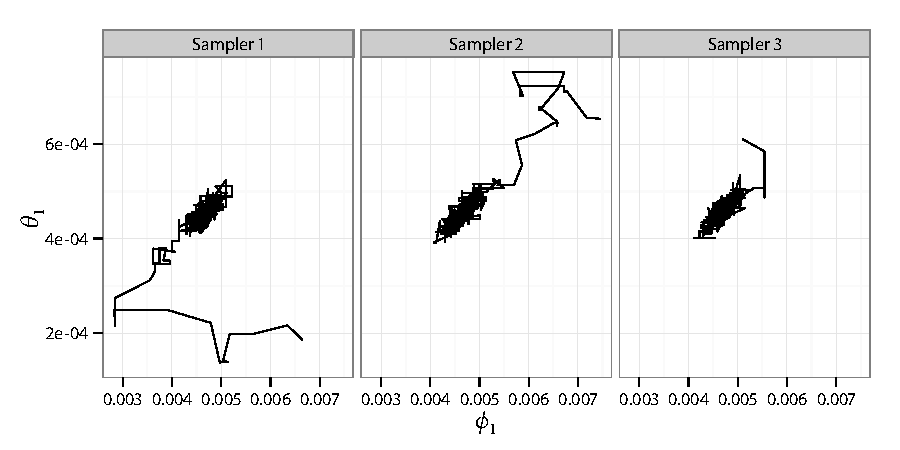
\includegraphics[width=\linewidth]{fig_src/PET_MH_Path.pdf}
  \caption[Traces of parameters in the random walk algorithm for the
  \protect\pet compartmental model (calibrated)]
  {Trace of $(\phi_1,\theta_1)$ from three random walk Metropolis-Hastings
  samplers for the one-compartments \pet model with non-informative priors,
  using well tuned proposal scales. The first few values of each trace is not
  shown in the plots since they are far away from the high probability region
  with an order of magnitude difference in values.}
  \label{fig:pet mh tuned}
\end{figure}

\begin{figure}[t]
  \UseAltLinespread
  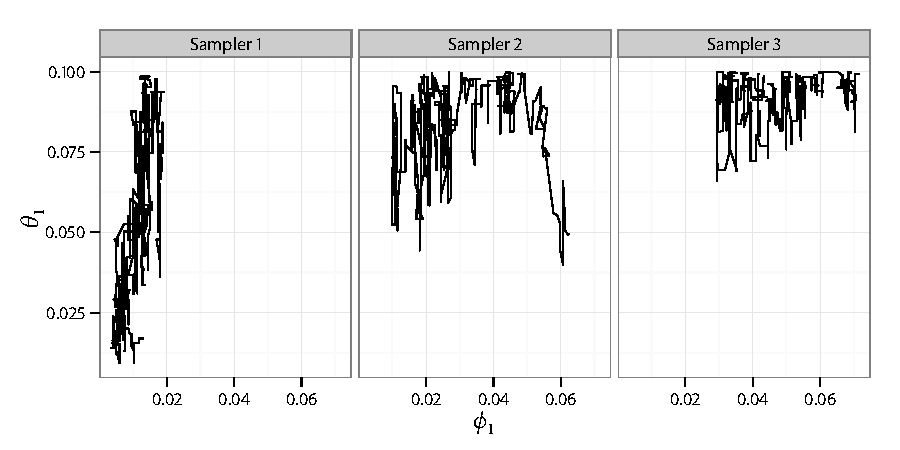
\includegraphics[width=\linewidth]{fig_src/PET_MH_H_Path.pdf}
  \caption[Traces of parameters in the random walk algorithm for the
  \protect\pet compartmental model (uncalibrated)]
  {Trace of $(\phi_1,\theta_1)$ from three random walk Metropolis-Hastings samplers for the one-compartments \pet model with non-informative priors, using proposal scales five times of those tuned.}
  \label{fig:pet mh untuned}
\end{figure}


\paragraph{Optimal proposal scales}

As seen in the above example, finding the optimal scales for a random walk
algorithm can be important for realistic applications. One way to measure the
optimality of the random walk is based on the asymptotic behavior of an
\emph{efficiency criterion} equal to the ratio of the variance of an
estimator based on an i.i.d\ sample and the variance of the estimator
$\hat\varphi_{\mcmc}^N$ in Equation~\eqref{eq:mcmc est}. In
\cite{Roberts:1997dg} it was recommended that the optimal proposal
distribution should produce chains with acceptance rate close to $0.5$ for
models with dimension $1$ or~$2$ and~$0.25$ for models with higher
dimensions. One of the more widely used type of proposals is the Normal
distribution or its multivariate variant. In \cite{Gelman:1995vx} a form of
optimal covariance is given as $(2.38^2/d)\Sigma_{\pi}$, where $d$ is the
dimension of the target distribution $\pi$ and $\Sigma_{\pi}$ is the true
covariance matrix of the parameters under $\pi$. In \cite{Roberts:2001ta} it
was further established that when the dimension goes to infinity, and the
covariance matrix is assumed to be diagonal, say $I_d\sigma_d^2$, the optimal
scaling of $\sigma_d$ has a corresponding acceptance rate $0.234$. This
optimal rate has been commonly used as a rule of thumb in practice. Some more
recent results for other proposal distributions including non-Gaussian cases
can be found in, e.g., \cite{Chris:2009vx,Peter:2011vx}

\subsubsection{Adaptive proposals}
\label{ssub:Adaptive proposals}

It often requires substantial efforts to tune an algorithm's proposals towards
optimality. Alternatively, many adaptive strategies have been developed. See
\cite{Andrieu:2008kh} for a recent review. The basic theme is that a family of
proposal distributions, indexed by some parameter, say $q(\cdot|x) =
q(\cdot|x, \theta)$ with $\theta\in\Theta$, is considered. And the value of
the parameter is updated along with the state. This leads to
Algorithm~\ref{alg:adaptive rw}.

\begin{algorithm}
\begin{algorithmic}
  \tophrule
  \STATE Draw $X^0\sim\mu$ where $\mu$ is the initial condition.
  \STATE Set $\theta^0$ to an arbitrary valid value.
  \STATE Set $t\leftarrow0$.
  \REPEAT
      \STATE Compute $\theta^t = \gamma^t(\theta^0,X^0,\dots,X^{t-1})$ where
      $\gamma^t$ is a transformation that update the parameters based on past
      samples.
      \STATE Draw $X^{t + 1}$ using the proposal $q(\cdot|x^t,\theta^t)$ with
      the Metropolis-Hastings rule.
      \STATE Set $t\leftarrow t+1$.
  \UNTIL{The accept rate of the last $K$ iterations are close to $0.234$.}
  \STATE Set $\theta\leftarrow\theta^t$.
  \STATE Perform Algorithm~\ref{alg:mh} with proposal $q(\cdot|x) =
  q(\cdot|x,\theta)$.
  \bottomhrule
\end{algorithmic}
\caption{Adaptive Metropolis-Hastings algorithm}
\label{alg:adaptive rw}
\end{algorithm}


There are many methods of updating the parameters. See \cite{Andrieu:2008kh}
for some common algorithms. One of the more widely used is based on the
Normal random walk or its multivariate variant. In
\cite{Haario:1999dh,Haario:2001gu}, it is proposed to use the past samples to
approximate the optimal covariance matrix $(2.38^2/d)\Sigma_{\pi}$
\cite{Gelman:1995vx}. The algorithm first initialize $\mu^0$, a $d$-vector
and $\Sigma^0$, a covariance matrix. At time $t$, they are updated with,
\begin{align}
  \mu^{t+1} &= \mu^t + \gamma^{t+1} (X^{t+1} - \mu^t) \\
  \Sigma^{t+1} &= \Sigma^t + \gamma^{t+1}((X^{t+1} - \mu^t)(X^{t+1} - \mu^t)^T
  - \Sigma^t)
\end{align}
where $\{\gamma^t\}_{t>0}$ is a sequence of small numbers, which are formally
arbitrary but could influence the performance. As noted by
\cite{Andrieu:2008kh}, though it is possible to set the sequence to a
constant $\gamma$, it is more common to set it to a deterministic decreasing
sequence such that $\sum_{t\ge1}\gamma^t = \infty$ and
$\sum_{t\ge1}(\gamma^t)^2<\infty$ to allow the effect of adaptation becomes
smaller and smaller as the algorithm progresses. This algorithm has also been
studied by \cite{Andrieu:2006tw} and others.

One obvious problem with such adaptive scheme is that the resulting chains
are no longer Markovian. And the limiting distribution, if it exists, may no
longer be $\pi$ as shown by examples in \cite{Andrieu:2008kh}. It is a common
practice to adapt the algorithm up to some point $t$, and stop the adaptation
and use parameter $\theta^t$ for all iterations onwards, as seen in
Algorithm~\ref{alg:adaptive rw}. The first part of the generated chain is
called the \emph{burn-in period} and is usually discarded afterwards.
Estimations are based on iterations after the burn-in period. Some rules for
when to stop adaptation was discussed in \cite{Andrieu:2008kh} and references
therein. There are more advanced techniques where the adaptive scheme attains
a vanishing adaptation property. Informally, after a long enough period, the
adaptive algorithm will only change the parameter $\theta$ slightly and
eventually it becomes stable. These algorithms require more careful design
to assure convergence.

Adaptive schemes are often necessary for realistic applications. For example,
consider the \pet compartmental model. As seen earlier, the scaling of the
Normal random walk influences the performance greatly. However, in a single
\pet scan, there are about a quarter of a million data sets, each results in
a different posterior surface. Manual tuning for each of them is a difficult
task. When the random walk algorithm is applied for the real data, we used
the adaptive Normal random walk for the parameters
$(\phi_{1:r},\theta_{1:r})$. Using 10,000 iterations as the burn-in period
for adaptation, we were able to obtain satisfactory acceptance rates (in the
range from $0.2$ to $0.4$) for the majority of the vast amount of data sets.

\subsection{Gibbs sampling}
\label{sub:Gibbs sampling}

The Metropolis-Hastings algorithm is generic in the sense that it requires
minimal knowledge of the target distribution to construct a valid sampler
(though not necessarily an efficient one). There also exists a class of \mcmc
algorithms that are more model dependent and they can use the (conditional)
features of the target distribution to construct potentially more efficient
samplers. One more important of them is the \emph{Gibbs sampling}. As we will
see later, it is a special case of the Metropolis-Hastings algorithm.

A Gibbs sampler, as first introduced by \cite{Geman:1993bp}, assumes that the
random variable $X$ can be written as $X = (X_1,\dots,X_p)$, where $X_i$'s are
either unidimensional or multidimensional. Let $\pi_1,\dots,\pi_p$ denote the 
\emph{full conditionals}, defined by
\begin{equation}
  X_i|x_1,\dots,x_{i-1},x_{i+1},\dots,x_p
  \sim \pi_i(x_i|x_1,\dots,x_{i-1},x_{i+1},\dots,x_p).
\end{equation}
If sampling from each of these distributions is possible, the associated
Gibbs sampler is given by the following algorithm that transits $X^t$ to
$X^{t+1}$ in $p$ steps. At each step $i$ (within one iteration), $X_i^{t+1}$
is generated from $\pi_i$,
\begin{equation}
  X_i^{t+1} \sim
  \pi_i(x_i^{t+1}|x_1^{t+1},\dots,x_{i-1}^{t+1},x_{i+1}^t,\dots,x_p^t).
\end{equation}
This leads to Algorithm~\ref{alg:gibbs}. See \cite[][chap.~9
and~10]{Robert:2004tn} for a full theoretical treatment of the Gibbs sampling.

\begin{algorithm}
\begin{algorithmic}
  \tophrule
  \STATE Draw $X^0\sim\mu$ where $\mu$ is the initial condition.
  \STATE Set $t\leftarrow0$.
  \REPEAT
    \FOR{$i = 1,\dots,p$}
      \STATE Draw
      $X_i^{t+1}\sim\pi_i(x_i|x_1,\dots,x_{i-1},x_{i+1},\dots,x_p)$.
    \ENDFOR
    \STATE Set $t\leftarrow t+1$.
  \UNTIL{Sufficient many samples have been produced.}
  \bottomhrule
\end{algorithmic}
\caption{Gibbs sampling (deterministic scan)}
\label{alg:gibbs}
\end{algorithm}


The Markov chain produced by a Gibbs sampler is irreducible if $\pi$
satisfies the so-called \emph{positivity condition}: All $\pi_i$ are positive
implies that $\pi$ is also positive \cite[][Theorem~10.8]{Robert:2004tn}. An
easier to verify condition for Harris recurrent is that the transition kernel
associated with Algorithm~\ref{alg:gibbs} is absolutely continuous with
respect to $\pi$ \cite{Tierney:1994uk}. Some simpler conditions can be found
in \cite{Hobert:1997vx}. Stronger convergence results such as geometrically
ergodicity are more difficult to be established for the Gibbs sampling in
general.

Intuitively, the decomposition of the joint distribution gives a particular
coordinate system with each step only exploring one of the coordinates. It
may take many cycles for the sampler to move around the surface of the joint
distribution. As shown in \cite[][note~9.7.1]{Robert:2004tn}, poor
parameterizations or decomposition can lead to slow convergence to the extent
of getting into a trapping state. This kind of situations most commonly occur
when two highly correlated parameters, say $X_{k_1}$ and $X_{k_2}$, are
updated in separate Gibbs moves. When $X_{k_1}$ is updated, because of its
dependency on $X_{k_2}$, its move is limited, and \emph{vice versa}.

For a particular parameterization of the target distribution, one can use
better decompositions to speedup convergence in a Gibbs sampler. There are
few general methodologies to solve this problem. The practical rule is to
create decompositions as independent as possible. For instance, in the
special case that $(X_1,\dots,X_p)$ are mutually independent, then a Gibbs
sampler is equivalent to sampling directly from the target distribution.
Admittedly, such decompositions, though they exist, can hardly be found in
interesting cases, otherwise one would not need to consider an \mcmc
algorithm in the first place.

Another approach is to reparameterize the target distribution with the same
principle of decomposition. For example, in
\cite[][sec.~10.4.1]{Robert:2004tn}, an example is given for a bivariate
Normal distribution. To sample $(X_1,X_2)$ from $\calN_2(0, \Sigma)$, where
$\Sigma$ is such that its eigenvalues satisfy $\lambda_{\text{\textsc{min}}}
\ll \lambda_{\text{\textsc{max}}}$ and its eigen vectors correspond to the
first and second diagonals of $\Real^2$, using a Gibbs sampler operating on
$(X_1 + X_2, X_1 - X_2)$ is much faster than that on $(X_1,X_2)$. The
reparameterization here is based on the eigen basis in this example. Note
that, this kind of techniques is not unique to the Gibbs sampling. They can
also be used for other \mcmc algorithms. See, e.g.,
\cite{Hills:1993vb,Gilks:1996vx} for more discussions on this topic.

\paragraph{Relation with the Metropolis-Hastings algorithm}

The Gibbs sampling can be viewed as a special case of the Metropolis-Hastings
algorithm. It is equivalent to a composition of Metropolis-Hastings samplers
in which at each step a single component is updated using its full conditional
as the proposal distribution. It is easy to verify that the acceptance
probability is uniformly equal to one \cite[][Theorem~10.13]{Robert:2004tn}.
Let $Y = (X_{1:i-1},Y_i,X_{i+1:p})$ where $Y_i$ is the value proposed with
$\pi_i$ at step $i$. The acceptance probability is then,
\begin{equation*}
  \alpha(x,y) = \min\Curly[bigg]{
    \frac{\pi(y)}{\pi(x)}
    \frac{\pi_i(x|x_{1:i-1},x_{i+1:p})}{\pi_i(y|x_{1:i-1},x_{i+1:p})},1}.
\end{equation*}
Rewrite $\pi(x)$ and $\pi(y)$ in the form of conditional densities, it follows
\begin{align*}
  \alpha(x,y) &= \min\Curly[bigg]{
    \frac{\pi_i(y_i|x_{1:i-1}, x_{i+1:p})\pi(x_{1:i-1},x_{i+1:p})}
    {\pi_i(x_i|x_{1:i-1}, x_{i+1:p})\pi(x_{1:i-1},x_{i+1:p})}
    \frac{\pi_i(x_i|x_{1:i-1}, x_{i+1:p})}{\pi_i(y_i|x_{1:i-1}, x_{i+1:p})},1}
    \\
  &= \min\{1,1\} = 1
\end{align*}

\paragraph{Random scan}

Algorithm~\ref{alg:gibbs} is also called the \emph{deterministic scan} Gibbs
sampling, in the sense that the components are updated in a deterministic
order $(X_1,\dots,X_p)$. Consequentially, this resulting chain is not
reversible. Another way of doing Gibbs sampling is to use a \emph{random
scan} \cite{Liu1995Gibbs}, where at each time $t$, a sequence of integers
$(k_1,\dots,k_p)$ is generated, usually uniformly across all permutations of
$(1,\dots,p)$, and the components are updated in the order of
$(X_{k_1},\dots,X_{k_p})$. This leads to Algorithm~\ref{alg:gibbs random}.
The resulting Markov chain is reversible \cite{Liu1995Gibbs}. This property
can be useful when applying the Central Limit Theorem
\cite[][sec.~10.1.2]{Robert:2004tn}.

\begin{algorithm}
\begin{algorithmic}
  \tophrule
  \STATE Draw $X^0\sim\mu$ where $\mu$ is the initial condition.
  \STATE Set $t\leftarrow0$.
  \REPEAT
    \STATE Draw $(k_1,\dots,k_p)\sim\sigma(1,\dots,p)$ where $\sigma$ is
    typically a distribution uniform over all permutations of $(1,\dots,p)$.
    \FOR{$i = 1,\dots,p$}
      \STATE Draw
      $X_{k_i}^{t+1}\sim
      \pi_{k_i}(x_{k_i}^{t+1}|
      x_{k_1}^{t+1},\dots,x_{k_{i-1}}^{t+1},x_{k_{i+1}}^t,\dots,x_{k_p}^t)$.
    \ENDFOR
    \STATE Set $t\leftarrow t+1$.
  \UNTIL{Sufficient many samples have been produced.}
  \bottomhrule
\end{algorithmic}
\caption{Gibbs sampling (random scan)}
\label{alg:gibbs random}
\end{algorithm}


\paragraph{Completion}

A common difficulty of the Gibbs sampling is that some of the full
conditionals may not be easily sampled from. In some situations, the full
conditionals of the target are not explicit at all. For example, missing data
models are often in the form,
\begin{equation*}
  f(\data|\theta) = \int f(\data, \mathbfit{z}|\theta)\intd \mathbfit{z}.
\end{equation*}
where $\mathbfit{z}$ is the unobserved data and $f(\data,\mathbfit{z}|\theta)$
is the likelihood function given the complete data $(\data,\mathit{z})$. In
these situations, it is possible to use \emph{completion} to construct a Gibbs
sampler. A distribution, say $\eta$ with the following property is chosen,
\begin{equation}
  \int\eta(x,y)\intd y = \pi(x).
\end{equation}
In other words, $\pi$ is a marginal of $\eta$. Then the Gibbs sampler is
constructed with the full conditionals of $\eta$ instead of $\pi$. The
sub-chain of the resulting Markov chain that corresponds to the marginal
$\pi$ is then $\pi$-invariant. When such a technique is used, there are many
possible choices of $\eta$ to complete $\pi$. Some applications provide
natural choices, such as the aforementioned missing data models.

\subsection{Reversible jump \protect\mcmc}
\label{sub:Reversible jump mcmc}

The reversible jump \mcmc (\rjmcmc) algorithm, introduced by
\cite{Green:1995dg}, is a technique widely used for simulations where the
dimension of the parameter space is not fixed. In the context of Bayesian
model selection, it can be used for inference of the full posterior
$\pi(\theta_k,\calM_k|\data)$, which is defined on the space $\Theta =
\bigcup_{k\in\calK}(\{\calM_k\}\times\Theta_k$). Situations where this can be
reduced to the estimation of the Bayes factor (Section~\ref{sub:Bayes
factor}), techniques reviewed so far in this chapter can be used. However,
when $\calK$ is (infinite) countable, or for other reasons, direct inference
on the full posterior distribution is desired, \rjmcmc is the most widely
used technique. The \rjmcmc and other algorithms that are capable of
simulating the full posterior distribution are not only conceptually
appealing, but also sometime necessary. In the scenarios where a large number
of models are possible and it is difficult to narrow down it to a manageable
set of candidate models, using \rjmcmc can be potentially more efficient than
performing simulations for each model when model selection is of interest.

The \rjmcmc algorithm adapts the Metropolis-Hastings algorithm to construct
transition kernels to simulate the full posterior. Instead of a single type
of moves defined by a proposal distribution, a countable set of moves are
considered, say $m\in\calM$. Each type of moves is capable of moving the
current state of the Markov chain between, say $\Theta_k$ and $\Theta_{k'}$,
the parameter space of model $\calM_k$ and $\calM_{k'}$ (where in the case of
$k = k'$, the move is similar to those in an \mcmc algorithm on a fixed
dimension space). At state $\theta_k\in\Theta_k$, a move type $m$ together
with a new state $\theta_{k'}\in\Theta_{k'}$ are proposed according to
$q_m(\theta_{k'}|\theta_k)r_m(\theta_k)$, where $r_m(\theta_k)$ is the
probability of choosing type $m$ move when at state $\theta_k$; and
$q_m(\theta_{k'}|\theta_k)$ is the proposal kernel for the new state when a
move of type $m$ is made. Usually, these moves are designed in pairs. For
type of moves $m$, there is an inverse type, say $m'$, that can move the
state $\theta_{k'}\in\Theta_{k'}$ to $\theta_k\in\Theta_k$. The move is
accepted with probability,
\begin{equation}
  \alpha(\theta_k,\theta_{k'}) =
  \min\Curly[bigg]{1,
    \frac{\pi(M_{k'})\pi(\theta_{k'}|M_{k'})p(\data|\theta_{k'},M_{k'})}
    {\pi(\calM_k)\pi(\theta_k|\calM_k)p(\data|\theta_k,\calM_k)}
    \frac{q_{m'}(\theta_k|\theta_{k'})r_{m'}(\theta_{k'})}
    {q_m(\theta_{k'}|\theta_k)r_m(\theta_k)}
  }.
\end{equation}
In practice, the proposed new state $\theta_{k'}$ is often implemented by
drawing a vector of continuous random variables, say $u$, independent of
$\theta_k$ and a deterministic bijection of vector $(\theta_k,u)$ to
$\theta_{k'}$, say $\theta_{k'} = T(\theta_k,u)$. The inverse of the move
from $\theta_{k'}$ back to $\theta_k$, $m'$, then uses the inverse of this
transformation. Through a simple change of variable, the conditional density
$q_m(\theta_{k'}|\theta_k)$ can be expressed in terms of the density of
vector $u$, say $q(u)$. The acceptance probability becomes
\begin{equation}
  \alpha(\theta_k,\theta_{k'}) =
  \min\Curly[bigg]{1,
    \frac{\pi(M_{k'})\pi(\theta_{k'}|M_{k'})p(\data|\theta_{k'},M_{k'})}
    {\pi(\calM_k)\pi(\theta_k|\calM_k)p(\data|\theta_k,\calM_k)}
    \frac{r_{m'}(\theta_{k'})}{r_m(\theta_k)}
    \frac{1}{q(u)}\Abs[bigg]{\frac{\partial\theta_{k'}}{\partial(\theta_k,u)}}
  },
\end{equation}
where the last term is the determinant of the Jacobian transformation. The
design of efficient between-model moves is often difficult, and the mixing of
these moves largely determines the performance of the algorithm.

It should be noted that, in the above we only described the move that
transits the parameters from the space of one model into another. As
mentioned earlier, in practice, \rjmcmc moves are designed in pairs. In each
pair, the two moves are capable of moving the parameters between two models.
For each type of move that transit the parameters from $\theta_k$ to
$\theta_{k'}$, an inverse move can be constructed. At each iteration, there
may be multiple steps. One step is to update the parameters without changing
the model. Other steps may move the parameters between models. At each of the
later step, a pair of moves is implemented, and with equal probabilities
(i.e., $r_m(\theta_k) = r_{m'}(\theta_k') = 0.5$), one type of the move in
the pair is performed.

The main difficulties lie in the choice of cross-model proposals and the
bijection $T$. Though the mapping $T$ theoretically is quite flexible, its
creation and optimization can be quite difficult in practice. This is
particularly true when the parameter space is complicated. In some extreme
cases, creating a valid kernel is already difficult. For example, in
multimodal models, where \rjmcmc has gain substantial attention, information
available in posterior distributions of any given model does not characterize
modes that exist only in models of higher dimension; and thus a successful
between-model move between these dimensions becomes difficult
\cite{Jasra:2007id}. Inefficient proposals result in Markov chains that are
slow to explore the whole parameter space. However, the natural ideas of
neighborhood and others, which proved to be useful concepts for within model
simulations, may no longer be intuitive in the variable dimension model
settings. For instance, when a cross-model occurs, the previous state of the
parameters, which may be in a high probability region of the model in the
last iteration, when transformed might be in a low probability region of the
model of the current iteration. In addition, \rjmcmc does not characterize
all models well as some may be visited by the chain only rarely. This may not
be a problem when the model is indeed of low posterior probability and there
is little interest in such models. However, in some cases it will be
difficult to determine whether the low acceptance rates of between model
moves results from actual characteristics of the posterior or from a poorly
adapted proposal kernel.

Some discussion of the optimization of the cross-model moves can be found in
\cite{Green:2009tr}. Also the adaptive scheme for the Metropolis-Hastings
algorithm has been extended for \rjmcmc, for example \cite{Hastie:2005vi}.
However little other work is known for the actual performance of this kind
of improvement to \rjmcmc. In \cite{Green:2001tk} a method called
\emph{delayed rejection} was discussed. In this method, a rejection of a
proposal does not immediately lead to the acceptance of current state,
instead a second proposal is attempted. Their numerical results showed
efficiency improvement but with increased computation cost.

\subsection{Population \protect\mcmc}
\label{sub:Population mcmc}

Population-based methods have been considered in recent research. An entire
family of such algorithms, sequential Monte Carlo, is considered in
Chapter~\ref{cha:Sequential Monte Carlo for Bayesian Computation}. Another
algorithm, population \mcmc, which has seen applications in the area of
Bayesian model comparison, is reviewed in this section.

Population \mcmc operates by constructing a sequence of distributions
$\{\pi_t\}_{t=0}^T$ with at least one of them being the target distribution
$\pi$. Parallel \mcmc chains are simulated for each of these distributions.
In addition, the chains interact with each other by swapping or crossover
moves, which allows fast mixing chains to ``lend'' information to slow mixing
chains. The outputs are therefore samples that approximate the product
$\prod_{t=0}^T\pi_t$ with the target distribution being a marginal.

Different choices of the sequence of distributions are possible. One commonly
used in practice is called tempering. For a target $\pi$, a sequence
$\{\pi_t\}_{t=0}^T$ is constructed such that,
\begin{equation}
  \pi_t(x) \propto [\pi(x)]^{\alpha(t/T)}
\end{equation}
where the mapping $\alpha:[0,1]\to[0,1]$ is monotonically increasing with
$\alpha(1) = 1$ (also see \cite{Marinari:1992vx} for similar annealing
schemes). Other similar schemes can be constructed. For example, in the
context of Bayesian modeling where $\pi$ is the posterior distribution
$\pi(\theta_k|\data,\calM_k) \propto
\pi(\theta_k|\calM_k)f(\data|\theta_k,\calM_k)$, one can construct a sequence
\begin{equation}
  \pi_t(\theta_k) =
  \pi(\theta_k|\calM_k)[f(\data|\theta_k,\calM_k)]^{\alpha(t/T)}
  \label{eq:power post}
\end{equation}
where the monotonically increasing mapping $\alpha$ satisfies $\alpha(0) = 0$
and $\alpha(1) = 1$. Therefore the sequence of distributions moves smoothly
from the prior, which usually can be sampled from easily, into the posterior.

The algorithm targets the distribution $\prod_{t=0}^T\pi_t$. After
initializing $T$ Markov chains for each of the marginals $\{\pi_t\}_{t=0}^T$
with a common support $E$, at each iteration, two types of moves are
performed. One is \emph{local} moves, sometimes termed \emph{mutation}, that
advances each chain individually using an \mcmc algorithms such as the
Metropolis-Hastings algorithm or the Gibbs sampling. One may select one chain
at random in each iteration to mutate or advance all chains in parallel. The
other type is \emph{global} moves. The purpose is to allow fast mixing chains
to transfer information into slowly mixing chains. In each global move, two
chains, say with indices $k_1$ and $k_2$, are selected. Let $X_{k_1}$ and
$X_{k_2}$ denote their current states. Two new states, $Y_{k_1}$ and
$Y_{k_2}$ are proposed according to conditional distributions
$q_{k_1}(y_{k_1}|x_{k_2})$ and $q_{k_2}(y_{k_2}|x_{k_1})$, respectively. That
is, the proposed new state of each chain depends on the current state of the
other. The new states are accepted with the usual Metropolis-Hastings
acceptance probability. This leads to Algorithm~\ref{alg:pmcmc}. There are
several approaches of the global move \cite{Jasra:2007in}. Two more widely
used are the following.

\begin{algorithm}
\begin{algorithmic}
  \tophrule
  \FOR{$k = 0,\dots,T$}
    \STATE Draw $X_k^0\sim\mu_k$ where $\mu_k$ is the initial condition.
  \ENDFOR
  \STATE Set $t\leftarrow0$.
  \REPEAT
    \STATE Draw $k_1$ from a uniform distribution on $(0,\dots,T-1)$. Set
    $k_2\leftarrow k_1 + 1$.
    \STATE Draw $Y_{k_1}^t\sim q_{k_1}(y_{k_1}^t|x_{k_2}^t)$ and
    $Y_{k_2}^t\sim q_{k_2}(y_{k_2}^t|x_{k_1}^t)$
    \STATE Compute $\alpha = \min\Curly[bigg]{
      \frac{\pi_{k_1}(y_{k_1}^t)\pi_{k_2}(y_{k_2}^t)
        q_{k_1}(x_{k_2}^t|y_{k_1}^t)q_{k_2}(x_{k_1}^t|y_{k_2}^t)}
      {\pi_{k_1}(x_{k_1}^t)\pi_{k_2}(x_{k_2}^t)
        q_{k_1}(y_{k_1}^t|x_{k_2}^t)q_{k_2}^t(y_{k_2}^t|x_{k_1}^t)}, 1}$
    \STATE Draw $U\sim\calU[0,1]$.
    \IF{$U\le\alpha$}
      \STATE Set $X_{k_1}^{t+1}\leftarrow Y_{k_1}^t$, $X_{k_2}^{t+1}\leftarrow
          Y_{k_2}^t$.
    \ELSE
      \STATE Set $X_{k_1}^{t+1}\leftarrow X_{k_1}^t$, $X_{k_2}^{t+1}\leftarrow
          X_{k_2}^t$.
    \ENDIF
    \FOR{$k = 0,\dots,T$}
      \STATE Draw $X_k^t\sim K_k(x_k^{t-1},x_k^t)$ where $K_k$ is a
      $\pi_k$-invariant Markov kernel.
    \ENDFOR
    \STATE Set $t\leftarrow t+1$.
  \UNTIL{Sufficiently many samples have been produced.}
  \bottomhrule
\end{algorithmic}
\caption{Population \mcmc with parallel updating.}
\label{alg:pmcmc}
\end{algorithm}


\paragraph{Exchange}

The exchange move selects two chains at random, say $k_1$ and $k_2$, and
propose to exchange the states between them. That is, the proposal
distribution $q_{k_1}(y_{k_1}|x_{k_2})$ is defined by
$\Pr(Y_{k_1}=x_{k_2}|x_{k_2}) = 1$ (similarly for
$q_{k_2}(y_{k_2}|x_{k_1})$). The proposed exchange is accepted or rejected
according to the Metropolis-Hastings acceptance probability,
\begin{equation}
  \alpha(x_{k_1}, x_{k_2}) =
  \min\Curly[bigg]{
  \frac{\pi_{k_1}(x_{k_2})\pi_{k_2}(x_{k_1})}
  {\pi_{k_1}(x_{k_1})\pi_{k_2}(x_{k_2})}, 1}.
  \label{eq:exchange accept}
\end{equation}
For this to work, usually the two chains are chosen such that they are
adjacent to each other in the sense that one is chosen randomly and the other
is selected to be the one most close to it. For example, in the tempering
scheme, usually a chain with index $k_1 \in\{0,1,\dots,T-1\}$ is chosen
randomly and it is proposed to be exchanged with the chain with index $k_2 =
k_1 + 1$. The delayed rejection approach in \cite{Green:2001tk} (see
Section~\ref{sub:Reversible jump mcmc}) can also be used in the exchange
moves. Thus two chains in some sense that are very different can also be
chosen. In either case, the key is that the chains chosen to be exchanged are
chosen uniformly over all chains.

\paragraph{Crossover}

Another type of global move, called crossover was mentioned in
\cite{Liang:2001dc}. Instead of proposing to exchange the whole states
$X_{k_1}$ and $X_{k_2}$, after the two chains are chosen, only parts of the
two states are proposed to be exchanged. Suppose the state $X$ can be
partitioned into $X = (X_1,\dots,X_p)$ in the same way for each chain. Then a
random position, say $l$ is chosen and the position $l$ of $X_{k_1}$ is
proposed to be exchanged with its counter-part in $X_{k_2}$. The acceptance
probability is the same as Equation~\eqref{eq:exchange accept} with suitable
notation changes. Let $X_{k_i} = (X_{k_i,1},\dots,X_{k_i,p})$ for $i = 1$
and~$2$ denote the current states and
\begin{align*}
  X_{k_1}' &= (X_{k_1,1},\dots,X_{k_1,l-1},
  X_{k_2,l},X_{k_1,l+1},\dots,X_{k_1,p}) \\
  X_{k_2}' &= (X_{k_2,1},\dots,X_{k_2,l-1},
  X_{k_1,l},X_{k_2,l+1},\dots,X_{k_2,p})
\end{align*}
denote the proposed states. Then the acceptance probability is,
\begin{equation}
  \alpha(x_{k_1},x_{k_2},x_{k_1}',x_{k_2}') = \min\Curly[bigg]
  {\frac{\pi_{k_1}(x_{k_1}')\pi_{k_2}(x_{k_2}')}
  {\pi_{k_1}(x_{k_1})\pi_{k_2}(x_{k_2})},1}
  \label{eq:cross accept}
\end{equation}
In \cite{Jasra:2007in} it was found that the cross over move can be more
efficient than the exchange move.

Population \mcmc algorithm can be more efficient than simulating from a
single chain. Consider the situation where the \mcmc algorithm targeting
distributions $\pi_1$ and $\pi_2$ might be trapped. If $\pi_1$ and $\pi_2$
are similar in the sense of the shape of the locations of local modes. And
each of them are trapped within different modes. The global move, say the
exchange move, proposes to exchange the values from one high probability
region with those in another high probability region. It is more likely that
such an exchange is accepted than the \mcmc algorithm jumps into the other
modes itself. Those chains that mix fast can explore the parameter space more
efficiently than those mix slower and are more likely to visit all the high
probability regions. Through the global moves they propose values in other
high probability regions to slowly mixing chains to help them avoid
trapping states.

\paragraph{Optimal placement of distributions}

As discussed earlier, population \mcmc allows efficient simulation of
previously difficult problem, though at a cost of increasing computational
cost. However, the algorithm requires another layer of optimization in
addition to the mixing speed of each local move -- the placement of the
sequence of distributions $\{\pi_t\}_{t=0}^T$. If too many chains are
present, the information can take many global moves to transfer from fast
mixing chains to slowly mixing ones. If there are too few chains and they are
placed far apart from each other, the global moves are likely to have small
acceptance rates. In \cite{Atchade:2010ha}, based on the idea of maximizing
the average information exchanged at each iteration, it was recommended that
an optimal placement of the distributions should have an global acceptance
rate around $0.234$. The optimal placement of the distributions can be
obtained iteratively if $\{\pi_t\}_{t=0}^T$ belongs to a family of
distributions, say $\pi_{\alpha} = \pi(\cdot|\alpha)$, indexed by $\alpha$.
The algorithm first finds $\alpha_0$ and $\alpha_1$ such that the population
\mcmc algorithm operating on $\{\pi_{\alpha_t}\}_{t=0}^1$ has a global
acceptance rate close to $0.234$. For example, if a tempering scheme is used,
one can set $\alpha_0 = 0$ and use a binary search algorithm to find
$\alpha_1$ since the smaller $\alpha_1$, the higher the acceptance rate. The
algorithm proceeds in the same way to find $\alpha_t$ for $t>1$.

\subsection{Convergence diagnostic}
\label{sub:Convergence diagnostic}

One important issue of \mcmc algorithms is their speed of convergence. It is
well understood yet sometime over looked in practice. In the previous
sections we demonstrated for many algorithms, under fairly general
conditions, the chains produced are ergodic, or even geometrically ergodic
(random walk). In some cases the chain can be uniformly ergodic (independent
Metropolis-Hastings algorithm). However, such development provides little
insight on how many iterations the algorithm should be run to produce
accurate estimates.

Convergence of an \mcmc algorithm is assessed by monitoring certain
statistics of samples. This process is also called \emph{convergence
diagnostic}. There are two types of convergence
\cite[][chap.~12]{Robert:2004tn} widely used in practice. As we will see
later, a convergence diagnostic can at best determine that a chain has not
converged yet. One cannot be certain that a chain does converge.

\subsubsection{Convergence to the stationary distribution}
\label{ssub:Convergence to the stationary distribution}

It might seem that a minimal requirement for samples from an \mcmc algorithm
to be used to approximate a target distribution $\pi$, is that the chain
converges to this stationary distribution. However, $\pi$ is only the limiting
distribution and the stationarity is at best achieved asymptotically.
Nonetheless, one possible assessment of such convergence is to obtain bounds
on the total variation norm,
\begin{equation*}
  \Norm{K^n(x,\cdot)-\pi}_{TV}
\end{equation*}
where $K^n(x,\cdot)$ is the distribution of samples at the $n$\xth iteration.
However, obtaining analytical bounds can be prohibitively difficult.

\paragraph{Graphical approach}

A natural empirical approach is to draw plots of simulated samples to detect
non-stationary behaviors. For instance, \cite{Gelfand:1990it} drew sequence
of the samples $\{X^t\}_{t\ge1}$ against the time $t$, which is a
functionality now commonly seen in softwares that implement \mcmc
algorithms.

It should be emphasized that, even when the plots appears to show stationary
behavior, it is still possible that the algorithm has not converged or
explored the support of the target distribution surface efficiently. For
example, consider the three-compartments \pet model and non-informative
priors without ordering (that is, parameters such as $(\phi_1,\theta_1)$ and
$(\phi_2,\theta_2)$ are exchangeable, see Section~\ref{sec:Application to
positron emission tomography}). We use one of the real data set and
constructed a random walk algorithm (see Section~\ref{sub:Metropolis-Hastings
algorithm}). Figure~\ref{fig:pet diag} shows the trace and histogram plots of
parameter $\theta_1$. It appears that the \mcmc chain has converged well.
However, from the properties of the model, it is known that this parameter
has at least three local modes. In fact, this sampler has been trapped into
one of them. In Figure~\ref{fig:pet diag c} the trace and histogram plots of
the same sampler but with better calibrated proposal scales are shown.

\begin{figure}[t]
  \linespread{1.1}\selectfont
  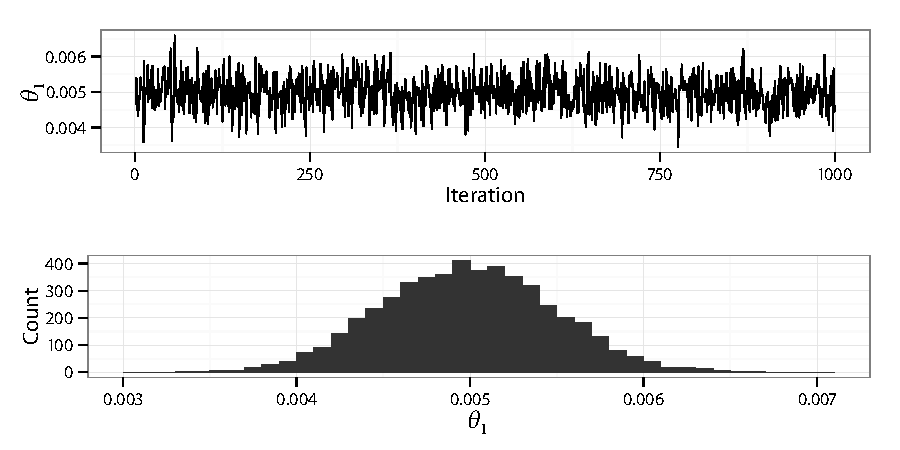
\includegraphics[width=\linewidth]{fig_src/PET_MH_Diag}
  \caption[Trace and histogram of parameters in the random walk algorithm for
  the \protect\pet compartmental model (calibrated)]
  {Trace and histogram plots of parameter $\theta_1$ from a \mcmc
    sampler for \pet model with three components and non-informative priors
    without ordering. The trace plot has 1,000 samples and the histogram plot
    has 10,000 samples. The sampler is not well calibrated.}
  \label{fig:pet diag}
\end{figure}

\begin{figure}[t]
  \UseAltLinespread
  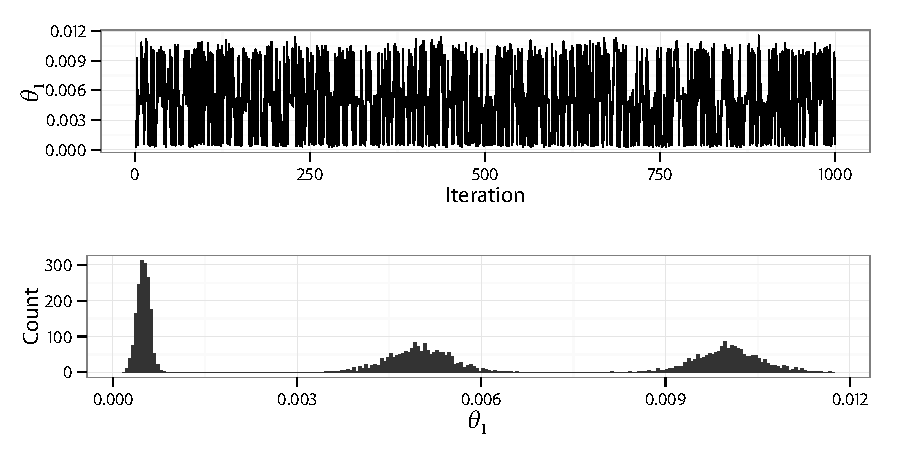
\includegraphics[width=\linewidth]{fig_src/PET_MH_Diag_C}
  \caption[Trace and histogram of parameters in the random walk algorithm for
  the \protect\pet compartmental model (uncalibrated)]
  {Trace and histogram plots of parameter $\theta_1$ from a \mcmc
    sampler for \pet model with three components and non-informative priors
    without ordering. The trace plot has 1,000 samples and the histogram plot
    has 10,000 samples. The sampler is well calibrated.}
  \label{fig:pet diag c}
\end{figure}


\paragraph{Non-parametric test}

Standard non-parametric tests can be applied in stationarity assessment. This
is based on the idea that, if the chain is stationary, then $X^{t_1}$ and
$X^{t_2}$ have the same distribution for any two arbitrary time points $t_1$
and $t_2$. Therefore standard tests can be used to compare the distribution of
samples $(X^t,\dots,X^{t+p-1})$ and $(X^{t+p},\dots,X^{t+2p})$. It should be
noted that the correlations between samples should be taken into
consideration. One solution is to use sub-samples. A \emph{batch size} $G$ is
introduced. Quasi-independent samples
$(X^{t_1+G},X^{t_1+2G},\dots,X^{t_1+pG})$ and
$(X^{t_2+G},X^{t_2+2G},\dots,X^{t_2+pG})$ are used to conduct the tests. See
\cite[][sec.~12.2.2]{Robert:2004tn} for some examples of such tests.

A simpler statistic to use, as seen in \cite{Gelman:2011vx}, is the ratio of
the variance of last few samples to that of all samples. Formally, for some
function $\varphi$, define the following ratio,
\begin{equation}
  R_T^N = \frac{\var[\varphi(X^{N-T+1},\dots,X^{N}]}
  {\var[\varphi(X^{1},\dots,X^{N}]}
\end{equation}
A value of $R_T^N$ between $0.9$ and $1.1$ was recommended. For example,
Figure~\ref{fig:pet diag ratio} shows the ratios of the variance of $V_D$
estimated using the final 1,000 samples to that of all 10,000 post burn-in
(the iterations used to adapt the sampler to optimal acceptance rates)
samples, for real \pet scan data sets. For the majority of data sets, the
ratios fall in the desired interval.

\begin{figure}[t]
  \linespread{1.1}\selectfont
  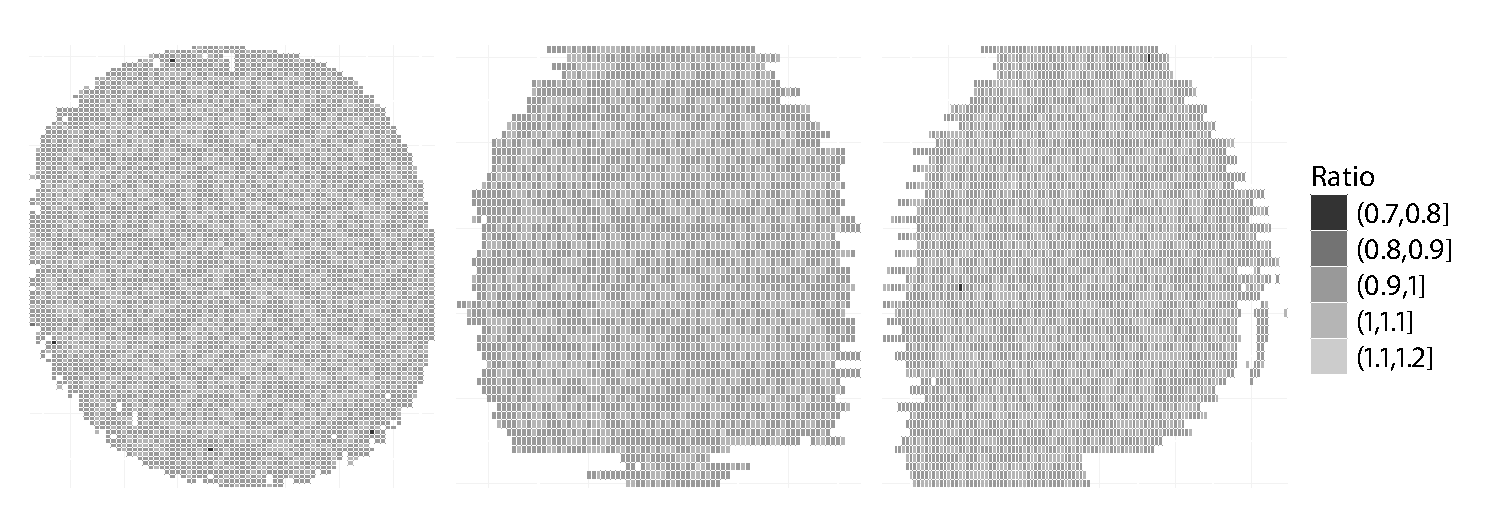
\includegraphics[width=\linewidth]{fig_src/PET_Converge}
  \caption[Convergence diagnostics for the random walk algorithm for the
  \protect\pet compartmental model using summary statistics]
  {Convergence diagnostics for the three-compartments \pet using ratio of
    variance of $V_D$ estimates using final 1,000 samples to that of all
    10,000 post burn-in samples.}
  \label{fig:pet diag ratio}
\end{figure}


\subsubsection{Convergence of averages}
\label{ssub:Convergence of averages}

In \cite{Yu:1998fn} it was proposed to use the cumulative sums and plot the
partial differences,
\begin{equation}
  D_N^t = \sum_{i=1}^t (\varphi(X^{(i)}) - S^N), \qquad t = 1,\dots,N,
\end{equation}
where
\begin{equation}
  S^N = \frac{1}{N}\sum_{i=1}^N \varphi(X^{(i)})
\end{equation}
is the final average. A simple variant of this method is to plot the average
of the first $t$ samples, $S^t$. The use of these quantities can be appealing
because they directly measure the stability of the estimator of interest. For
instance, Figure~\ref{fig:pet vd mean} shows the posterior mean estimate of
$V_D$ for a three-compartments \pet model. The posterior mean from five
samplers initialized with different values converge to the same value.

\begin{figure}[t]
  \UseAltLinespread
  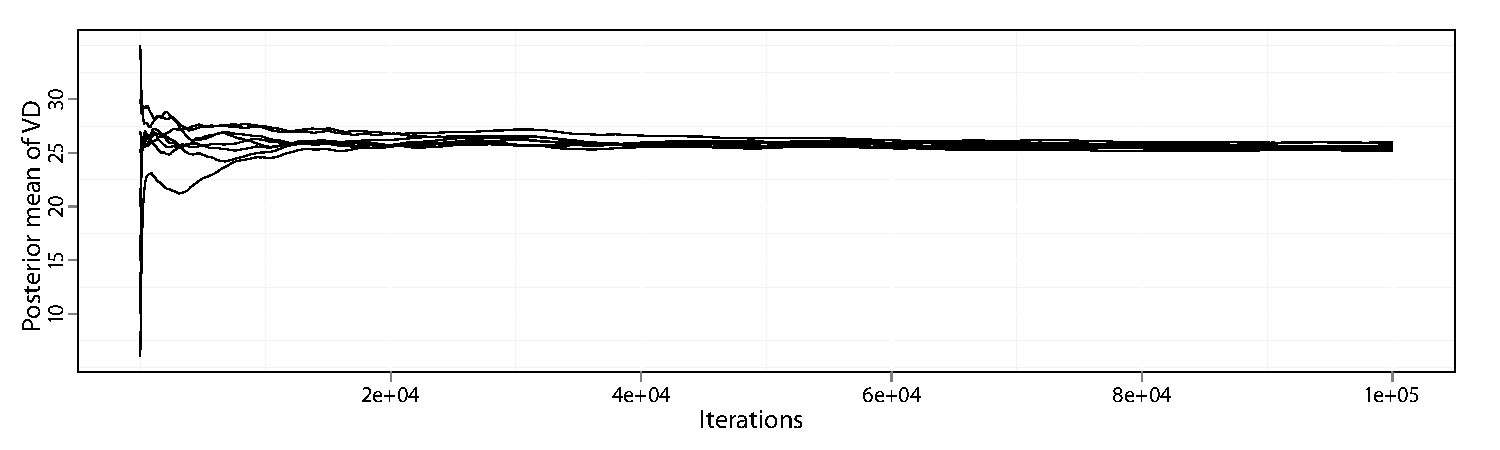
\includegraphics[width=\linewidth]{fig_src/PET_VD}
  \caption[Convergence diagnostics for the random walk algorithm for the
  \protect\pet compartmental model using averages]
  {Estimates of $V_D$ when starting the \mcmc chain from different
    values for a typical data set of a \pet model with three component.}
  \label{fig:pet vd mean}
\end{figure}


A more robust approach was proposed in \cite{Robert:1995ge}. The idea is to
use several convergent estimators based on the same samples. The chain is
first iterated until all estimators are close to each other in the sense that
the differences are smaller than a preset tolerance value. And then onwards
simulations are used for inferences. One obvious estimator is the empirical
average. Another one is similar to the importance sampling estimator,
\begin{equation}
  \varphi_{\mcmc-\is}^N
  = \sum_{i=1}^N \varphi(Y^{(i)})\frac{\pi(Y^{(i)})}{q(Y^{(i)}|X^{(i)})}
  \label{eq:sn is}
\end{equation}
where $\{Y^{(i)}\}_{i=1}^N$ are samples from $q(y^t|x^t)$, a distribution
that depends on the current state $X^t$. When the distributions are known
only up to some normalizing constants, then a variant similar to that in
Equation~\eqref{eq:is unnormalized} is used. Unlike the importance sampling
in Section~\ref{sec:Importance sampling}, this estimator is based on
dependent samples instead of i.i.d\ samples. However, as shown in
\cite[][Lemma~12.11]{Robert:2004tn}, the weighted terms in the sum are
uncorrelated.

In the particular case of the Gibbs sampling, the distribution,
\begin{equation}
  q(y^t|x^{t-1}) \propto
  \prod_{i=1}^p \pi_i(y_i^t|y_{1:i-1}^t,x_{i+1:p}^{t-1})
\end{equation}
is a natural choice to be used as the proposal distribution and samples from
Gibbs sampler can be used. In this case, $Y^{(i)} = X^{(i)}$.

For the generic Metropolis-Hastings algorithm, the samples simulated from the
proposal distributions (both those accepted and rejected) can be recycled to
calculate the importance sampling estimate. In this case, $Y^{(i)}$ is the
proposed value, $X^{(i)}$ are the accepted values and the distribution
$q(\cdot|x^t)$ is simply the proposal distribution. This approach is more
robust to trapping state than the simple plots of averages.

For example, consider an independent Metropolis-Hastings algorithm whose
proposal $\eta$ has only one high probability region $A$ while the target
$\pi$ has two high probability regions $A$ and $B$ such that $Pr(x\in
A)\approx\Pr(x\in B)$. The chain is likely to be trapped in $A$ and $S^N$
might appear to be stable. However, $\varphi_{\mh-\is}^N$ is much less stable
since those values occasionally proposed within $B$, though very likely to be
accepted, they also have extreme large value of the weight
$\pi(Y^{(i)})/\eta(Y^{(i)})$. This leads to large variance of estimator
$\varphi_{\mcmc-\is}^N$. In this case, $\varphi_{\mh-\is}^N$ is stable when
values of high target density values are also proposed frequently.

\subsection{Application to Bayesian model comparison}
\label{sub:MCMC Application to Bayesian model comparison}

It is clear that \rjmcmc can be used directly for the purpose of Bayesian
model selection, as it generates samples from the full posterior with the
model posterior distribution $\pi(\calM_k|\data)$ as a marginal.

For within model simulations, that is the algorithms generate Markov chains
targeting the posterior distribution $\pi(\theta_k|\data,\calM_k) \propto
f(\data|\theta_k,\calM_k)\pi(\theta_k|\calM_k)$, the dependent samples can be
used for the purpose of Bayesian model comparison for finite a set of models
through approximating the marginal likelihood and thus the Bayes factor, which
is the ratio of the marginal likelihood of two models. A few methods are
discussed here.

\subsubsection{Generalized harmonic mean estimator}
\label{ssub:Generalized harmonic mean estimator}

Recall that, the marginal likelihood is written as,
\begin{equation*}
  p(\data|\calM_k) = \int
  f(\data|\theta_k,\calM_k)\pi(\theta_k|\calM_k)\intd\theta_k.
\end{equation*}
For the purpose of simplicity, in this section we drop the dependency on the
model $\calM_k$ and simply write $p(\data) = \int
f(\data|\theta)\pi(\theta)\intd\theta$. With samples generated by an \mcmc
algorithm targeting the posterior distribution $\pi(\theta|\data) \propto
f(\data|\theta) \pi(\theta)$ available, say $\{\theta^{(i)}\}_{i=1}^N$, an
estimator of $p(\data)$ can be obtained by the harmonic mean
\cite{Newton:1994wm},
\begin{equation}
  \widehat{p(\data)}_{\hm}^N =
  \Round[bigg]{\frac{1}{N}\sum_{i=1}^N\frac{1}{f(\data|\theta^{(i)})}}^{-1}
\end{equation}
Unfortunately this estimator can suffer instability problem when samples with
small likelihoods are generated. In fact this estimator does not always have a
finite variance and therefore in general does not satisfy a Central Limit
Theorem (\clt). An improvement seen in \cite{Kass:1995vb} is,
\begin{equation}
  \widehat{p(\data)}_{\ghm}^N = \Round[bigg]{
    \frac{1}{N}\sum_{i=1}^N
    \frac{\gamma(\theta^{(i)})}{f(\data|\theta^{(i)})\pi(\theta^{(i)})}}^{-1},
\end{equation}
where $\gamma$ is a proper density function. This is based on the identity,
\begin{equation}
  \frac{1}{p(\data)}
  = \int \frac{\gamma(\theta)}{p(\data,\theta)}
  \frac{p(\data,\theta)}{p(\data)} \intd \theta
  = \int \frac{\gamma(\theta)}{p(\data,\theta)} \pi(\theta|\data) \intd \theta
\end{equation}
It can be seen that the distribution $\gamma$ plays a role similar to that of
the target distribution for the importance sampling in the sense that the
posterior distribution now acts as a proposal distribution. For similar
reasons, high efficiency is most likely to be obtained when $\gamma$ is
roughly proportional to $f(\data|\theta)$ \cite{Kass:1995vb}. The above
equation suggests that the estimator has a finite variance if the tails of
$\gamma$ are thin enough compared to the posterior distribution
$\pi(\theta|\data)$. In \cite{Gelfand:1994ux} the use of a multivariate Normal
distribution with moments approximated from the samples as a natural choice of
$\gamma$ was suggested. In addition, the variance of the estimator can also be
estimated for $1/\widehat{p(\data)}_{\ghm}^N$ from the posterior samples
through,
\begin{equation}
  \widehat{\var}\Square[bigg]{\frac{1}{\widehat{p(\data)}_{\ghm}^N}} =
  \frac{1}{N^2}\sum_{i=1}^N \Round[bigg]{
    \frac{\gamma(\theta^{(i)})}{f(\data|\theta^{(i)})\pi(\theta^{(i)})}
    - \frac{1}{\widehat{p(\data)}_{\ghm}^N}}^2.
\end{equation}
The above estimator provides a way of monitoring the convergence of the
estimator. Though more stable than the harmonic mean estimator
$\widehat{p(\data)}_{\hm}^N$, this generalized estimator still requires
considerable care in the implementation, especially the choice of the density
$\gamma$, to ensure good performance and indeed a finite variance estimator.

The method described above can be used for most \mcmc algorithms, such as the
Metropolis-Hastings algorithm, the Gibbs sampling and population \mcmc (by
only using the sub-chain that corresponds to the distribution of interest).

\paragraph{Results for \pet compartmental model}

We conclude the discussion on the generalized harmonic mean estimator with
results for the \pet compartmental model with real data. For a
$r$-compartments \pet model (see Section~\ref{sec:Application to positron
  emission tomography}), a Student $t$ distributed error structure (see
Section~\ref{sec:Error models}), and informative priors (see
Section~\ref{sub:Choice of priors}), we construct a random Metropolis-Hastings
algorithm with four blocks. Again, recall the parameterization in
Section~\ref{sec:Application to positron emission tomography},
\begin{enumerate}
  \item Update $\phi_{1:r}$ with a multivariate Normal random walk proposal.
  \item Update $\theta_{1:r}$ with a multivariate Normal random walk proposal.
  \item Update $\tau$ with a Normal random walk proposal on the logarithm
    scale, i.e., on $\log\tau$.
  \item Update $\nu$ with a Normal random walk proposal on the logarithm
    scale, i.e., on $\log\nu$.
\end{enumerate}
There is a 10,000 iterations used for adaptation (the burn-in period) and
10,000 iterations are used for estimation. Results in \cite{Zhou2013} showed
that the long burn-in period is more than enough for the majority of the
samplers to converge well. The generalized harmonic mean estimator
$\hat\varphi_{\ghm}^N$ is used to compute the Bayes factor. The model
selection results, along with those from \aic and \bic methods for the purpose
of comparison, are shown in Figure~\ref{fig:pet mo}. It can be seen that the
Bayesian model selection results shows more plausible structure than the
information criteria. With the information criteria, the distribution of the
model orders across the image appears to be more or less random while the
Bayesian results show some structure with more active regions within the brain
have higher order models. See also the discussions in \cite{Zhou2013} and
references therein.

\afterpage{\begin{figure}[t]
  \UseAltLinespread
  \centering
  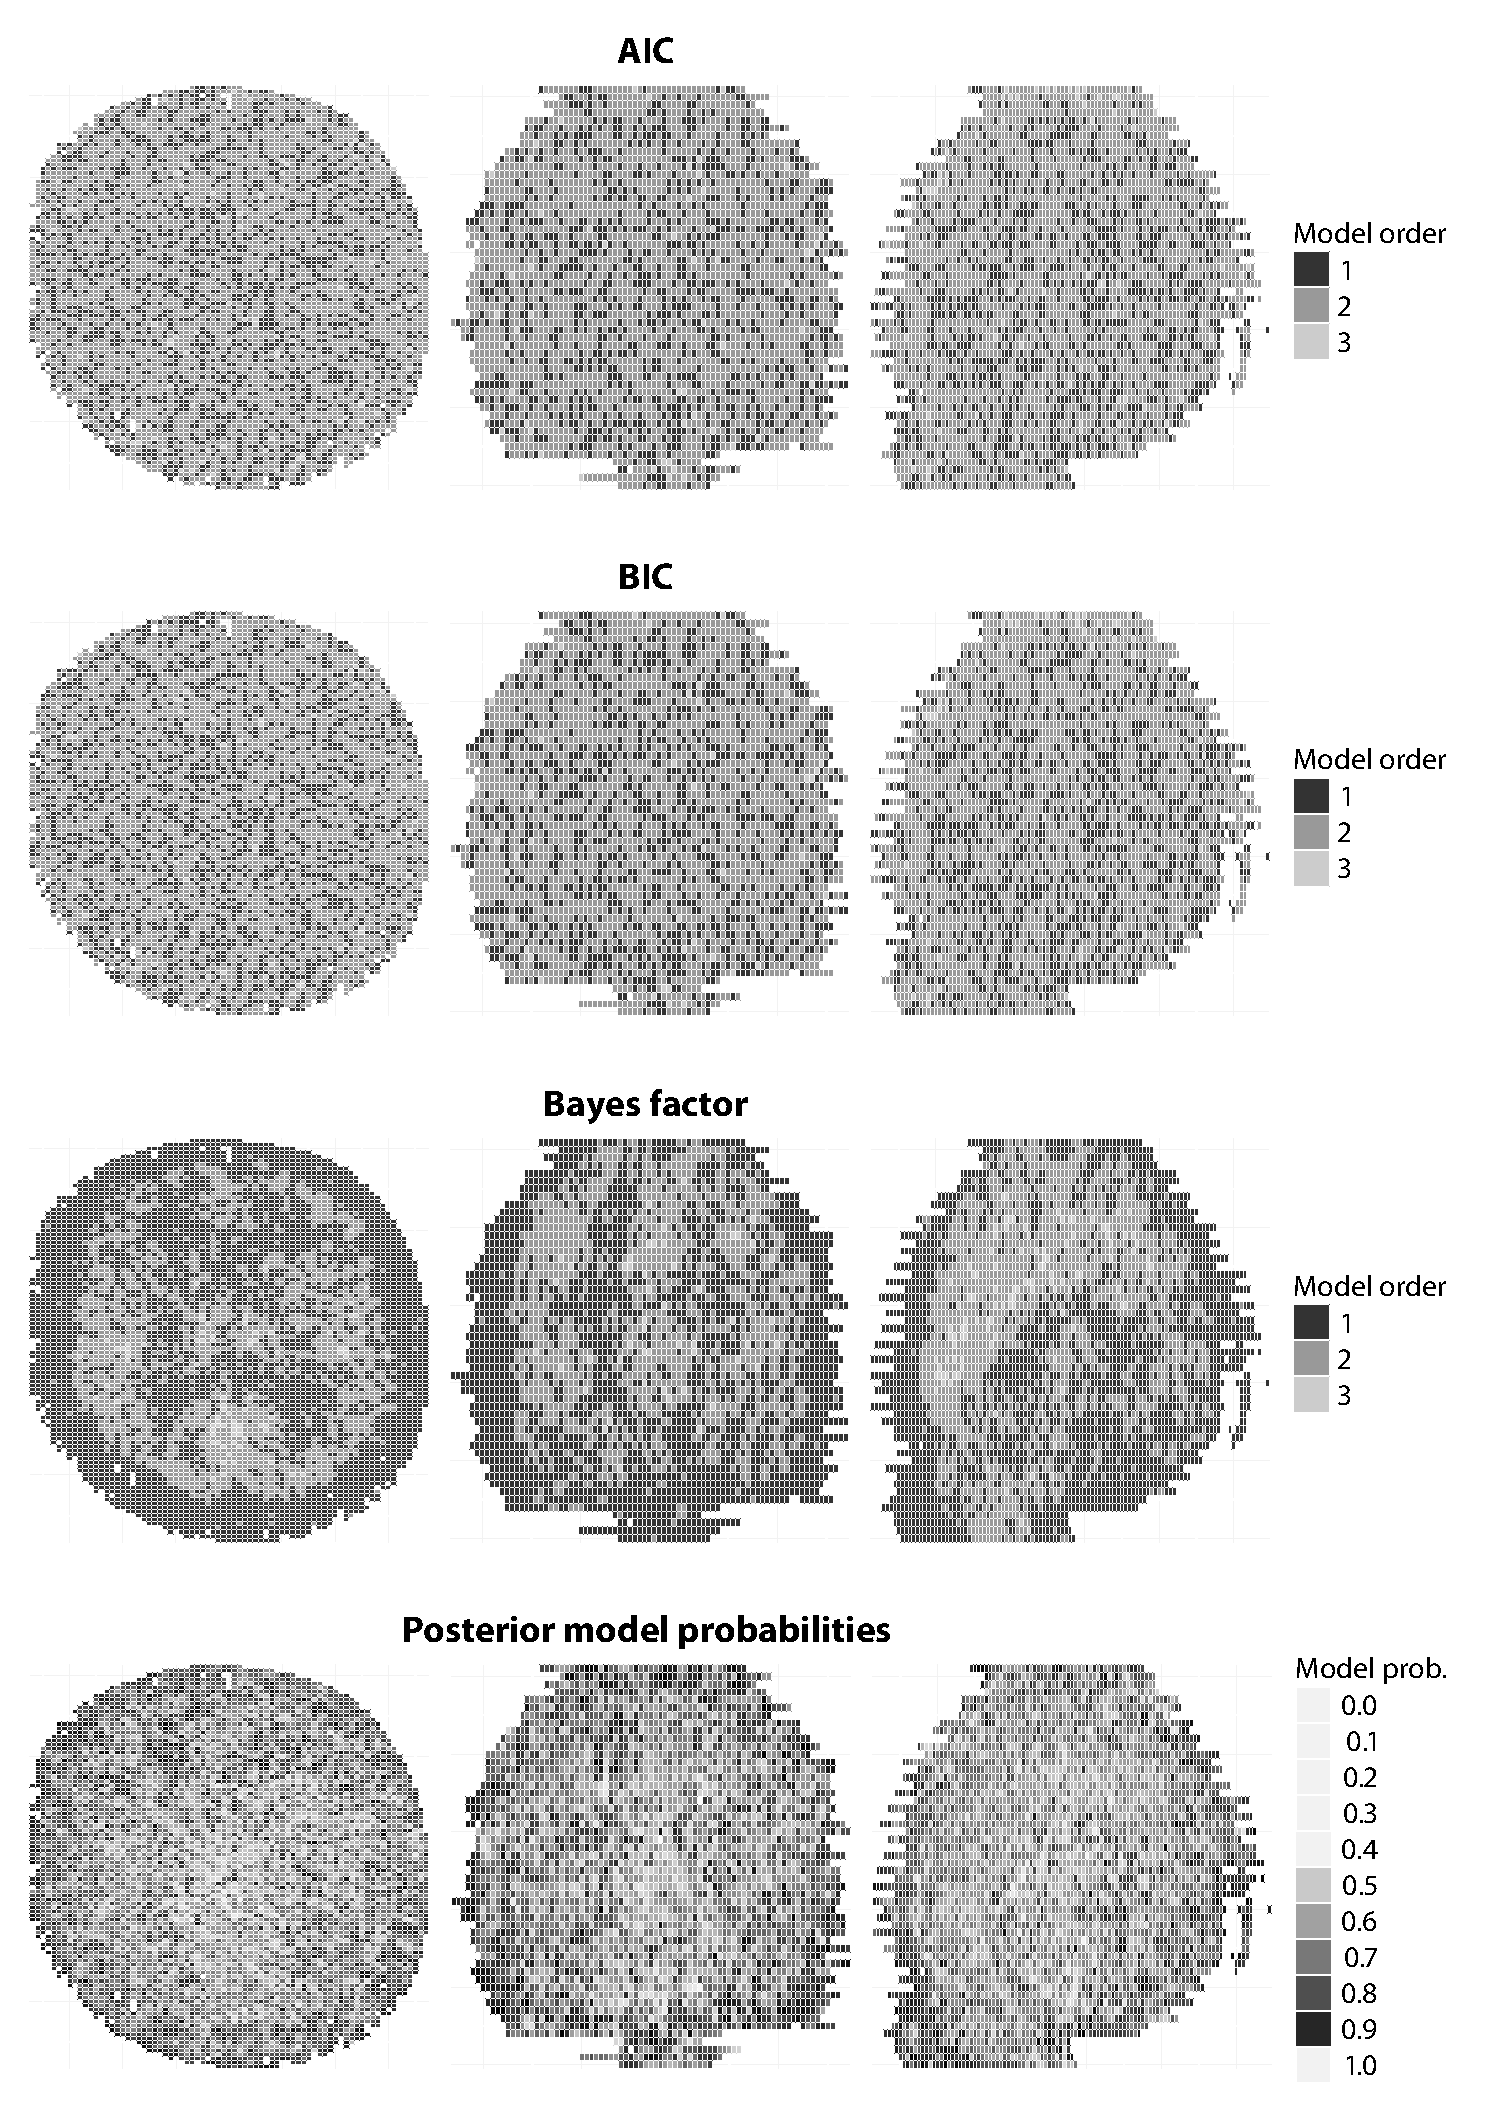
\includegraphics[width=0.95\linewidth]{fig_src/PET_MO}
  \caption[Model selection results for the \protect\pet compartmental model]
  {Model selection results for \pet model using real data set. From
    top to bottom: Model order selected by \aicc (see Section~\ref{sub:A
      second order aic}); Model order selected by \bic (see
    Section~\ref{sub:Bayes factor}); Model order selected by using Bayesian
    model comparison with marginal likelihood approximated by generalized
    harmonic mean estimator; The posterior model probability
    $\pi(\calM_k|\data)$ (see Section~\ref{sub:Model choice problems}) with
    uniform prior model probability $\pi(\calM_k)$.}
  \label{fig:pet mo}
\end{figure}
\clearpage}

The convergence results for this simulation were already shown in
Figure~\ref{fig:pet diag ratio}. It should be noted that, though as shown in
Figure~\ref{fig:pet vd mean}, accurate estimation of the parameter $V_D$ does
not really need this many iterations. However, accurate estimation of the
marginal likelihood requires considerably more samples.

\subsubsection{Estimator using the Gibbs sampling}
\label{ssub:Estimator using the Gibbs sampling}

In the particular case of the Gibbs sampling, \cite{Chib:1995em} provides an
alternative estimator based on that the identity,
\begin{equation}
  p(\data) = \frac{f(\data|\theta)\pi(\theta)}{\pi(\theta|\data)},
\end{equation}
holds for any value of $\theta$. Therefore an estimator can be obtained by
substituting $\theta$ with a specific value, say $\theta^*$, which is usually
chosen from the high probability region of the posterior distribution and
approximating the denominator using outputs from the Gibbs sampler.

Formally, assume it is possible to construct a Gibbs sampler for the
decomposition $\theta = (\theta_1,\dots,\theta_p)$. Write $\pi(\theta|\data)$
as,
\begin{equation}
  \pi(\theta|\data) = \pi(\theta_1|\data)
  \prod_{i=2}^p\pi(\theta_i|\data,\theta_{1:i-1})
\end{equation}
and given $\theta^*$, we have the estimator,
\begin{equation}
  \widehat{p(\data)}_{\gs}^N = \frac{f(\data|\theta^*)\pi(\theta^*)}
  {\pi(\theta_1^*|\data)
    \prod_{i=2}^p\pi(\theta_i^*|\data,\theta_{1:i-1}^*)}.
\end{equation}
The value of $\pi(\theta_1^*|\data)$, the marginal ordinate of
$\pi(\theta|\data)$ can be approximated with output from the Gibbs sampler.
For example,
\begin{equation}
  \hat\pi^N(\theta_1^*|\data)
  = \frac{1}{N}\sum_{i=1}^N \pi(\theta_1^*|\data,\theta_{2:p}^{(i)})
  \label{eq:est gibbs first}
\end{equation}
since
\begin{align*}
  \pi(\theta_1^*|\data)
  &= \int\pi(\theta_1^*, \theta_{2:p}|\data)\intd\theta_{2:p} \\
  &= \int\pi(\theta_1^*|\data,\theta_{2:p})
  \pi(\theta_{2:p}|\data)\intd\theta_{2:p} \\
  &= \Exp[\pi(\theta_1^*|\data,\theta_{2:p})|\data]
\end{align*}
where the expectation is taken with respect to the marginal distribution of
$\theta_{2:p}$ conditional on the data.

The term $\pi(\theta_i^*|\data,\theta_{1:i-1}^*)$ can be approximated based on
the identity,
\begin{align}
  \pi(\theta_i^*|\data,\theta_{1:i-1}^*)
  &= \int \pi(\theta_i^*,\theta_{i+1:p}|\data,\theta_{1:i-1}^*)
  \intd\theta_{i+1:p} \notag\\
  &= \int \pi(\theta_i^*|\data,\theta_{1:i-1}^*,\theta_{i+1:p})
  \pi(\theta_{i+1:p}|\data,\theta_{1:i-1}^*) \intd\theta_{i+1:p}
\end{align}
and using a Gibbs sampler operating on $\theta_{i:p}$ with
$\pi(\theta_{i:p}|\data,\theta_{1:i-1}^*)$ as the target distribution and an
estimator similar to that in Equation~\eqref{eq:est gibbs first}. This is
possible because all the full conditionals required to construct such a Gibbs
sampler can be sampled from, otherwise the original Gibbs sampler cannot be
constructed.

In addition to the usual requirement of a Gibbs sampler, that all the full
conditionals can be sampled from, this method also requires that all these
densities are known including their normalizing constants, and thus can be
computed point-wise. The advantage is that this estimator does not suffer
from the instability problem like the harmonic mean estimator and its
generalizations. Only averages of full conditionals are involved in the
calculation, which are less sensitive to extreme small values.

A generalization to the generic Metropolis-Hastings algorithm was provided by
\cite{Chib:2001gq}, where the proposal distributions are required to be
known including their normalizing constants.

\subsubsection{Population \mcmc with path sampling}
\label{ssub:Population mcmc with path sampling}

For population \mcmc, as proposed in \cite{Calderhead:2009bd}, a Monte Carlo
approximation to the path sampling estimator \cite{Gelman:1998ei} can be used
for the purpose of approximating the marginal likelihood. Given a parameter
$\alpha$ which defines a family of distributions, $\{\pi_{\alpha} =
\gamma_{\alpha}/Z_{\alpha}\}_{\alpha\in[0,1]}$ which moves smoothly from
$\pi_0 = \gamma_0/Z_0$ to $\pi_1 = \gamma_1/Z_1$ as $\alpha$ increases from
zero to one, one can estimate the logarithm of the ration of their
normalizing constants via a simple integral relationship,
\begin{equation}
  \log\Round[bigg]{\frac{Z_1}{Z_0}} = \int_0^1\Exp_{\pi_{\alpha}}
  \Square[bigg]{\frac{\diff\log\gamma_{\alpha}(X)}{\diff\alpha}}
  \intd\alpha.
  \label{eq:path integral}
\end{equation}
where the inner expectation is taken with respect to $\pi_{\alpha}$ and
$Z_{\alpha}$ is the normalizing constant for the unnormalized density
$\gamma_{\alpha}$. The path sampling estimator for the ratio of the
normalizing constants $Z_1$ and $Z_0$ are based on Monte Carlo approximations
of the above integration. One direct approach, as seen in \cite{Gelman:1998ei}
is to simulate samples $(\alpha,X)$ where $\alpha$ are uniformly distributed
on the interval $[0,1]$ and conditional on $\alpha$, $X$ is distributed with
$\pi_{\alpha}$. As we will see, with some modifications of the evaluation of
the outer integration, this estimator can be approximated using samples from
a population \mcmc.

There are various ways of constructing such a family of distributions, for
example, the sequence of distributions in Equation~\eqref{eq:power post},
$\alpha = \alpha(t/T)$. Population \mcmc provides samples that can be used
to approximate this path sampling estimator. Given samples
$\{X_0^{(i)},\dots,X_T^{(i)}\}_{i=1}^N$ from $N$ iterations of a population
\mcmc sampler, one can approximate the expectation under distribution
$\pi_{\alpha} = \pi_{\alpha(t/T)} = \pi_t$ by the empirical average of the
sub-chain $\{X_t^{(i)}\}_{i=1}^N$. The integration~\eqref{eq:path integral}
can be approximated with a numerical integration scheme such as the
Trapezoidal rule. This leads to the following estimator,
\begin{equation}
  \widehat{p(\data)}_{\ps}^N = \sum_{t=1}^T
  \frac{1}{2}(\alpha_t - \alpha_{t-1})(U_t^N + U_{t-1}^N)
\end{equation}
where $U_t^N$ is the estimate of
$\diff\log\gamma_{\alpha}(X)/\diff\alpha$ evaluated at $\alpha = \alpha_t$
using samples $\{X_t^{(i)}\}_{i=1}^N$.

As shown in \cite{Calderhead:2009bd}, the use of path sampling can reduce the
variance of the estimator significantly compared to the harmonic mean
estimator and its generalizations. However, the estimator
$\widehat{p(\data)}_{\ps}^N$ is biased because of the use of numerical
integration. It is clear that the smaller the interval
$[\alpha_{t-1},\alpha_t]$ (closer the distribution $\pi_{t-1}$ and $\pi_t$),
the smaller the bias. However, this can come into conflict with the
convergence speed of the population \mcmc algorithm. As discussed earlier, in
this setting, the global moves can potentially mix slowly. For example, for
the one-compartment \pet model and using the sequence of
distributions~\eqref{eq:power post}, the optimal placement that results in an
acceptance rate of globals close to $0.234$ has only six chains. The path
sampling estimate has a 60\% relative bias. With 30 chains and a sensible
placement, the bias can be reduced to be negligible. However, the global move
has an acceptance rate about $0.85$, which implies that the sampler is not
mixing well.

The use of path sampling for approximating the Bayes factor will be revisited
in Chapter~\ref{cha:Sequential Monte Carlo for Bayesian Computation} for
sequential Monte Carlo. More results for the \pet model and other examples can
also be found in the same chapter.

\section{Discussions}
\label{sec:Monte Carlo Discussion}

In this chapter, a few Monte Carlo algorithms have been reviewed. One of the
more important class of algorithms, Markov chain Monte Carlo has been widely
used for Bayesian modeling.

The Metropolis-Hastings algorithm provide a generic solution to a large array
of applications. There are established results for tuning the algorithm for
optimal performance. The Gibbs sampler can be more appealing when there are
decompositions of the parameter vector that lead to easy to sample full
conditionals. Both algorithms can benefit from reparameterization that leads
to more independent parameters. The difficulty of \rjmcmc is that the
cross-model move is often difficult to design. The population \mcmc algorithm
can provide robust solution for high dimensional multimodal problems where the
other algorithm may be inefficient due to the difficulty of exploring local
modes separated by small probability regions. Its performance depends on both
the design of the \mcmc algorithm that update each chain and the placement of
the sequence of distributions.

The \rjmcmc algorithm can be used for Bayesian model selection through the
simulation of the posterior model probabilities. It can be difficult to
implement though conceptually appealing. Other algorithms can be used to
approximate the marginal likelihood and thus the Bayes factor using various
estimators. The harmonic mean estimator and its generalizations can be
calculated for most \mcmc algorithms. However, they suffer stability issues.
For the Gibbs sampling and the Metropolis-Hastings algorithm, there exist
more stable estimators. However, they require knowledge of certain
distributions that are not always available. Population \mcmc can also use
the path sampling estimator. There is a trade-off between convergence speed
and the accuracy of the estimator in term of its bias.

It should be noted that, the application of Monte Carlo methods is not limited
to integration. They have also found application in areas such as optimization
(see \cite[][chap.~5]{Robert:2004tn} and references therein). In addition,
Monte Carlo integration is also not limited to the Bayesian paradigm. For
instance, Monte Carlo integration can be used for hypothesis tests when
various asymptotic assumptions, such as normality, are not suitable. For
examples, see \cite[][sec.~3.2]{Robert:2004tn} and references therein.

There are many other Monte Carlo algorithms not reviewed in this chapter.
Notable examples are slice sampling and perfect sampling (see \cite[][chap.~8
and~13]{Robert:2004tn}). Another class of algorithms, sequential Monte Carlo
(\smc) operates by iteratively construct efficient proposal distributions for
the importance sampling. A recent develop, particle \mcmc
\cite{Andrieu:2010gc} combines the strength of \mcmc and \smc by using \smc
samplers as proposal in the Metropolis-Hastings algorithm or the Gibbs
sampling. This chapter is far from a complete review of the topic on Monte
Carlo methods. The algorithms reviewed are widely used for the purpose of
Bayesian model comparison. They have become standard tools of statisticians
for Bayesian computation. In the next chapter, we will study the use of \smc
for this purpose in detail. Some novel algorithms will be introduced.
